%Este trabalho está licenciado sob a Licença Atribuição-CompartilhaIgual 4.0 Internacional Creative Commons. Para visualizar uma cópia desta licença, visite http://creativecommons.org/licenses/by-sa/4.0/deed.pt_BR ou mande uma carta para Creative Commons, PO Box 1866, Mountain View, CA 94042, USA.

\documentclass[12pt]{book}

\input ../preambulo.tex

\makeindex

\begin{document}

\frontmatter

\title{Matemática numérica}
\author{Pedro H A Konzen}
\date{\today}
\ifishtml
\else
\addcontentsline{toc}{chapter}{Capa}
\fi

\maketitle

%Este trabalho está licenciado sob a Licença Atribuição-CompartilhaIgual 4.0 Internacional Creative Commons. Para visualizar uma cópia desta licença, visite http://creativecommons.org/licenses/by-sa/4.0/ ou mande uma carta para Creative Commons, PO Box 1866, Mountain View, CA 94042, USA.

\chapter*{Licença}\label{licenca}
\addcontentsline{toc}{chapter}{Licença}

Este trabalho está licenciado sob a Licença Atribuição-CompartilhaIgual 4.0 Internacional Creative Commons. Para visualizar uma cópia desta licença, visite http://creativecommons.org/licenses/by-sa/4.0/deed.pt\_BR ou mande uma carta para Creative Commons, PO Box 1866, Mountain View, CA 94042, USA.



\chapter*{Prefácio}\label{prefacio}
\addcontentsline{toc}{chapter}{Prefácio}

O site \href{https://www.notaspedrok.com.br}{notaspedrok.com.br} é uma plataforma que construí para o compartilhamento de minhas notas de aula. Essas anotações feitas como preparação de aulas é uma prática comum de professoras/es. Muitas vezes feitas a rabiscos em rascunhos com validade tão curta quanto o momento em que são concebidas, outras vezes, com capricho de um diário guardado a sete chaves. Notas de aula também são feitas por estudantes - são anotações, fotos, prints, entre outras formas de registros de partes dessas mesmas aulas. Essa dispersão de material didático sempre me intrigou e foi o que me motivou a iniciar o site.

Com início em 2018, o site contava com apenas três notas incipientes. De lá para cá, conforme fui expandido e revisando os materais, o site foi ganhando acessos de vários locais do mundo, em especial, de países de língua portugusa. No momento, conta com 13 notas de aula, além de minicursos e uma coleção de vídeos e áudios.

As notas de \emph{Algoritmos e Programação I} fazem uma introdução a algoritmos e programação de computadores com a linguagem {\python}. É pensada para estudantes de cursos de matemática e áreas afins.

Aproveito para agradecer a todas/os que de modo assíduo ou esporádico contribuem com correções, sugestões e críticas. ;-)

\begin{flushright}
  Pedro H A Konzen\\\url{https://www.notaspedrok.com.br}
\end{flushright}



\tableofcontents
\addcontentsline{toc}{chapter}{Sumário}

\mainmatter



\chapter{Introdução}\label{cap_intro}

Vamos começar executando nossas primeiras \emph{linhas de código} na linguagem de programação {\python}. Em um \emph{terminal} {\python} digitamos

\begin{lstlisting}
>>> print('Olá, mundo!')
\end{lstlisting}

Observamos que \lstinline+>>>+ é o símbolo do \lstinline+prompt de entrada+ e digitamos nossa \emph{instrução} logo após ele. Para executarmos a instrução digitada, teclamos \lstinline+<ENTER>+. Uma vez executada, o terminal apresentará as seguintes informações

\begin{lstlisting}
>>> print('Olá, mundo!')
Olá, mundo!
>>> 
\end{lstlisting}

Pronto! O fato do símbolo de \lstinline+prompt de entrada+ ter aparecido novamente, indica que a instrução foi completamente executada e o terminal está pronto para executar uma nova instrução.

A \emph{linha de comando} executada acima pede ao computador para imprimir no \lstinline+prompt de saída+ a frase \lstinline+Olá, mundo!+. O \emph{método} {\PYTHONprint} contém instruções para imprimir \emph{objetos} em um dispositivo de saída, no caso, imprime a frase na tela do computador.

Bem! Talvez imprimir no \lstinline+prompt de saída+ uma frase que digitamos no \lstinline+prompt de entrada+ possa parecer um pouco redundante no momento. Vamos considerar um outro exemplo, computar a soma dos números ímpares entre $0$ e $100$. Podemos fazer isso como segue

\begin{lstlisting}
>>> sum([i for i in range(100) if i%2 != 0])
2500
\end{lstlisting}

Oh! No momento, não se preocupe se não tenha entendido a linha de comando de entrada, ao longo dessas notas de aula isso vai ficando natural. A linha de comando de entrada usa o método {\PYTHONsum} para computar a soma dos elementos da \emph{lista} de números ímpares desejada. A lista é construída de forma \emph{iterada} e \emph{indexada} pela \emph{variável} \lstinline+i+, para \lstinline+i+ no intervalo/faixa de $0$ a $99$, se o resto da divisão de \lstinline+i+ por $2$ não for igual a $0$. Ok! O resultado computado foi $2500$.

De fato, a soma dos números ímpares de $0$ a $100$
\begin{equation}
  (1, 3, 5, \dotsc, 99)
\end{equation}
é a soma dos 50 primeiros elementos da progressão aritmética $a_i = 1 + 2i$, $i=0, 1, \ldots$, i.e.
\begin{align}
  \sum_{i=0}^{49}a_i &= a_0 + a_1 + \cdots + a_{49}\\
                     &= 1 + 3 + \cdots + 99\\
                     &= \frac{50(1 + 99)}{2}\\
                     &= 2500
\end{align}
como já esperado! Em {\python}, esta última conta pode ser computada como segue

\begin{lstlisting}
>>> 50*(1+99)/2
2500.0
\end{lstlisting}

%Este trabalho está licenciado sob a Licença Atribuição-CompartilhaIgual 4.0 Internacional Creative Commons. Para visualizar uma cópia desta licença, visite http://creativecommons.org/licenses/by-sa/4.0/ ou mande uma carta para Creative Commons, PO Box 1866, Mountain View, CA 94042, USA.

\chapter{Aproximação por mínimos quadrados}\label{cap_ajuste}
\thispagestyle{fancy}

\section{Problemas lineares}\label{cap_ajuste_sec_prob_lin}

Dado um conjunto de $n$ pontos $\{(x_i,y_i)\}_{i=1}^n$, $x_i\neq x_j$ para $i\neq j$, e uma família de $m \leq n$ funções $\{f_i(x)\}_{i=1}^m$, o problema linear de aproximação por mínimos quadrados consiste em determinar os $m$ coeficientes $\{c_i\}_{i=1}^m$ tal que a função
\begin{align}    
  f(x;c) &= \sum_{j=1}^m c_jf_j(x) \\
         &= c_1f_1(x) + c_2f_2(x) + c_3f_3(x) + \cdots + c_mf_m(x)
\end{align}
aproxime o conjunto de pontos dados no sentido de mínimos quadrados, i.e. o vetor dos coeficientes $c = (c_1, c_2, \dotsc, c_m)$ é solução do seguinte problema linear de minimização
\begin{equation}
  \min_{c} \left\{E:= \sum_{i=1}^n (y_i - f(x_i;c))^2\right\}.
\end{equation}

A fim de trabalharmos com uma notação mais compacta, definimos o resíduo $r(c) = (r_1(c), r_2(c), \dotsc, r_n(c))$, onde $r_i(c) := y_i - f(x_i)$ e $c = (c_1, c_2, \dotsc, c_m)$. Com esta notação, o problema de mínimos quadrados se resume a resolver
\begin{equation}\label{eq:pmq}
  \min_{c} \{E := \|r(c)\|_2^2\}.
\end{equation}

\subsection{Método das equações normais}

A fim de resolver o problema de mínimos quadrados~\eqref{eq:pmq}, observamos que o erro quadrático
\begin{align}
  E &= \|r(c)\|_2^2 \\
    &= \sum_{i=1}^n r_i(c)^2 \\
    &= \sum_{i=1}^n \left(y_i - f(x_i;c)\right)^2 \\
    &= \sum_{i=1}^n \left(y_i - \sum_{j=1}^m c_jf_j(x_i)\right)^2 \\
    &= \|y - Ac\|_2^2,
\end{align}
onde $y = (y_1, y_2, \dotsc, y_n)$ e
\begin{equation}
  A :=
  \begin{bmatrix}
    f_1(x_1) & f_2(x_1) & \cdots & f_m(x_1) \\
    f_1(x_2) & f_2(x_2) & \cdots & f_m(x_2) \\
    \vdots & \vdots & \vdots & \vdots \\
    f_1(x_n) & f_2(x_n) & \cdots & f_m(x_n)
  \end{bmatrix}.
\end{equation}

Os parâmetros $c_j$ que minimizam o erro $E$ são solução do seguinte sistema de equações
\begin{equation}
  \frac{\p E}{\p c_j} = 2\sum_{i=0}^n r_i(c)\frac{\p}{\p c_j}r_i(c) = 0,
\end{equation}
onde $j=1, 2, \dotsc, m$. Ou, em uma notação mais apropriada,
\begin{align}
  \nabla_c E = 0 &\Leftrightarrow A^Tr(c) = 0\\
  &\Leftrightarrow A^T(y - Ac) = 0\\
  &\Leftrightarrow A^TAc = A^Ty.
\end{align}

Portanto, o problema linear de mínimos quadrados se resume em resolver as chamadas \emph{equações normais}\index{equações normais}
\begin{equation}\label{eq:equacoes_normais}
  A^TAc= A^Ty.
\end{equation}

Logo, o problema linear de mínimos quadrados~\eqref{eq:pmq} reduz-se a resolver o sistema linear \eqref{eq:equacoes_normais} para $c$. Isto nos leva a questão de verificar se $A^TA$ é invertível. De sorte, da disciplina de álgebra linear temos o seguinte teorema.

\begin{teo}
  A matriz $A^TA$ é positiva definida se, e somente se, as colunas de $A$ são linearmente independentes (i.e. $\text{posto}(A)=n$).
\end{teo}
\begin{dem}
  Se as colunas de $A$ são linearmente independentes, então $x\neq 0$ implica $Ax\neq 0$ e, equivalentemente, $x^TA^T\neq 0$. Portanto, $x\neq 0$ implica $x^TA^TAx = \|Ax\|_2^2 > 0$, o que mostra que $A^TA$ é positiva definida.

  Suponhamos, agora, que as colunas de $A$ não são linearmente independentes. Então, existe $x_0\neq 0$ tal que $Ax_0 = 0$. Mas, então, $x_0^TA^TAx_0=0$, o que mostra que $A^TA$ não é positiva definida. 
\end{dem}

Este teorema nos fornece uma condição suficiente para a existência (e unicidade) de solução do problema linear de mínimos quadrados. Mais especificamente, se as colunas da matriz $A$ são linearmente independentes, então os coeficientes da função $f(x)$ que melhor ajustam os pontos dados são
\begin{equation}
  c = (A^TA)^{-1}A^Ty.
\end{equation}

\begin{ex}\normalfont{(Ajuste de polinômios)}\label{ex:ajuste_de_polinomios}
  Considere o problema de ajustar o conjunto de pontos
  \begin{center}
    \begin{tabular}{l|rrrr}
      $i$ & $1$ & $2$ & $3$ & $4$ \\\hline
      $x_i$ & $-1$ & $0$ & $1$ & $1,5$\\
      $y_i$ & $1,2$ & $-0,1$ & $0,7$ & $2,4$\\\hline
    \end{tabular}
  \end{center}
  por um polinômio quadrático da forma
  \begin{equation}
    p(x) = p_1x^2 + p_2x + p_3
  \end{equation}
  no sentido de mínimos quadrados.  

  \begin{figure}[h]
    \centering
    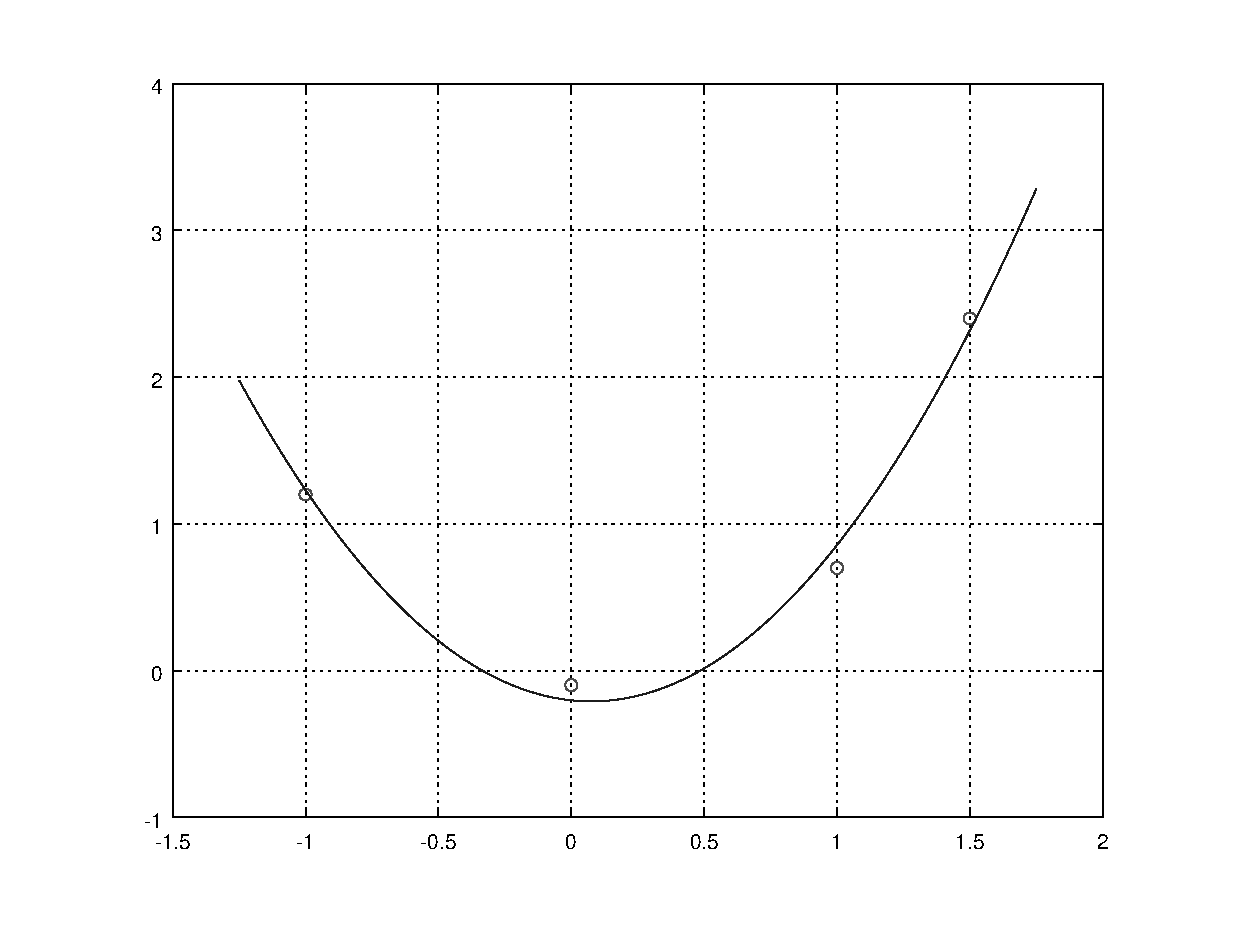
\includegraphics[width=\textwidth]{cap_ajuste/dados/ex_mq_poli/ex_mq_poli}
    \caption{Esboço do polinômio ajustado no Exemplo~\ref{ex:ajuste_de_polinomios}.}
    \label{fig:ex_mq_poli}
  \end{figure}
  
  
  Neste caso, a família de funções do problema de mínimos quadrados é $f_1(x) = x^2$, $f_2(x) = x$ e $f_3(x) = 1$. Assim sendo, os coeficientes $p = (p_1, p_2, p_3)$ são solução do seguinte sistema linear
  \begin{equation}\label{eq:aux3_md}
    A^TAp = A^Ty,
  \end{equation}
  onde $y = (y_1, y_2, y_3)$ e
  \begin{equation}
    A :=
    \begin{bmatrix}
      x_1^2 & x_1 & 1 \\
      x_2^2 & x_2 & 1 \\
      x_3^2 & x_3 & 1 \\
      x_4^2 & x_4 & 1
    \end{bmatrix}.
  \end{equation}
  Emfim, resolvendo as equações normais~\eqref{eq:aux3_md}, obtemos
  \begin{equation}
    p(x) = 1,25x^2 -0,188x - 0,203.
  \end{equation}
  A Figura~\ref{fig:ex_mq_poli} mostra um esboço dos pontos (em vermelho) e do polinômio ajustado (em azul).
  
  \ifisoctave
  Os coeficientes e um esboço do polinômio ajustado podem ser obtidos no \verb+GNU Octave+ com o seguinte código:
\begin{verbatim}
#pontos
x = [-1 0 1 1.5]';
y = [1.2, -0.1, 0.7, 2.4]';

#resol. as eqs. normais
A = [x.^2 x.^1 x.^0];
p = inv(A'*A)*A'*y

#esboco do pol. ajustado
xx = linspace(-1.25,1.75);
plot(x,y,'ro',...
     xx,polyval(p,xx));grid
\end{verbatim}
  \fi
  
\end{ex}


\begin{ex}\normalfont{(Ajuste de curvas)}\label{ex:ajuste_de_curvas}
  Consideremos o mesmo conjunto de pontos do exemplo anterior (Exemplo~\ref{ex:ajuste_de_polinomios}). Aqui, vamos ajustar uma curva da forma
  \begin{equation}
    f(x) = c_1\sen(x) + c_2\cos(x) + c_3
  \end{equation}
no sentido de mínimos quadrados. Para tanto, formamos a matriz
\begin{equation}
  A :=
  \begin{bmatrix}
    \sen(x_1) & \cos(x_1) & 1 \\
    \sen(x_2) & \cos(x_2) & 1 \\
    \sen(x_3) & \cos(x_3) & 1 \\
    \sen(x_4) & \cos(x_4) & 1
  \end{bmatrix}
\end{equation}
  e, então, resolvemos as equações normais $A^TAc = A^Ty$ para o vetor de coeficientes $c=(c_1, c_2)$. Fazendo isso, obtemos $c_1=-0,198$, $c_2=-2,906$ e $c_3=2,662$. A Figura~\ref{fig:ex_ajuste_de_curvas} mostra um esboço da curva ajustada (linha azul) aos pontos dados (círculos vermelhos).

  \begin{figure}[h]
    \centering
    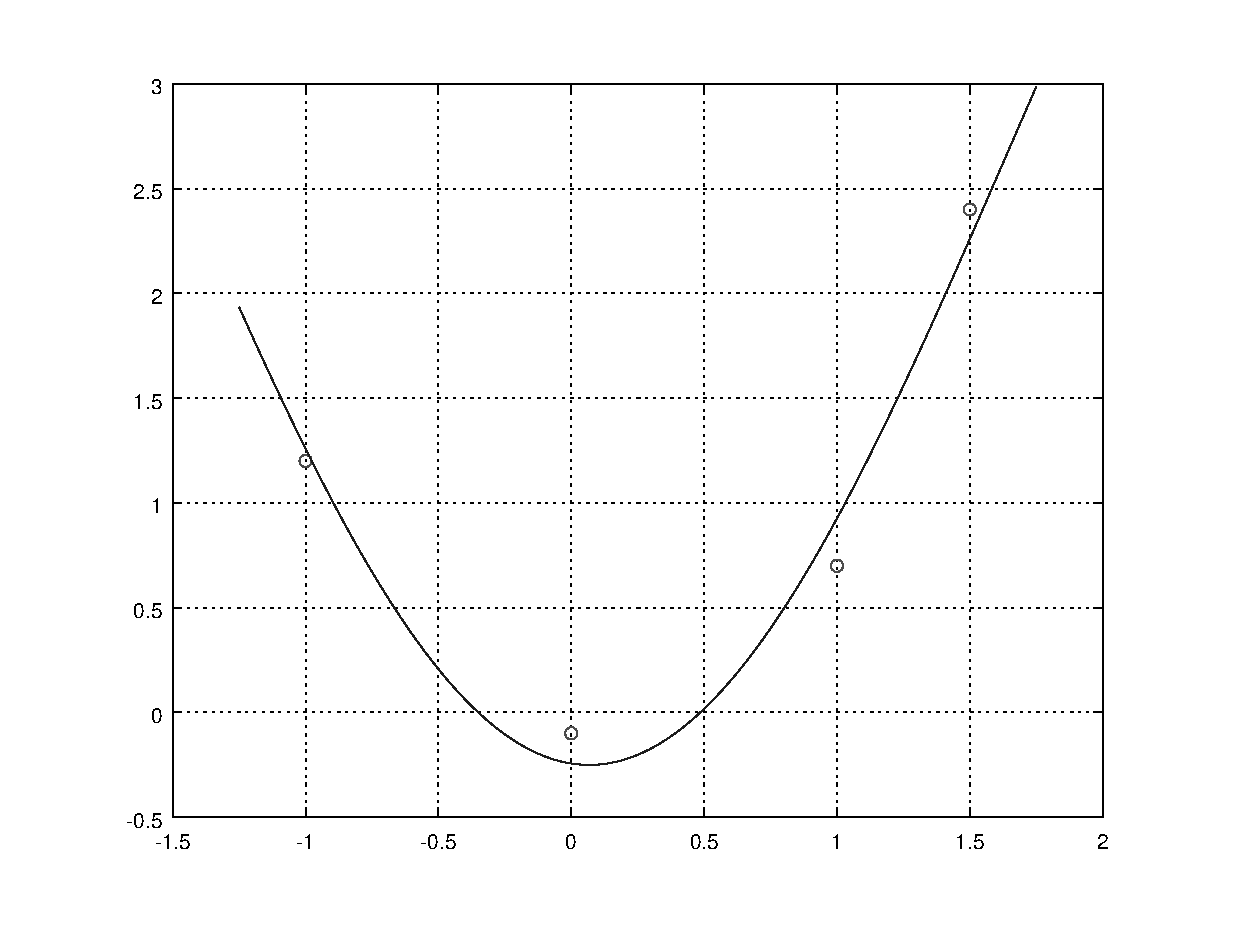
\includegraphics[width=\textwidth]{cap_ajuste/dados/ex_mq_curvas/ex_mq_curvas}
    \caption{Esboço da curva ajustada no Exemplo~\ref{ex:ajuste_de_curvas}.}
    \label{fig:ex_ajuste_de_curvas}
  \end{figure}

\ifisoctave
Os coeficientes e um esboço do polinômio ajustado podem ser obtidos no \verb+GNU Octave+ com o seguinte código:
\begin{verbatim}
#pontos
x = [-1 0 1 1.5]';
y = [1.2, -0.1, 0.7, 2.4]';

#resol. as eqs. normais
A = [sin(x) cos(x) ones(4,1)];
c = inv(A'*A)*A'*y

#curva ajustada
f = @(x) c(1)*sin(x) + c(2)*cos(x) + c(3)

#esboco da fun. ajustada
xx = linspace(-1.25,1.75);
plot(x,y,'ro',...
     xx,f(xx));grid
\end{verbatim}
\fi

\end{ex}

\begin{ex}\normalfont{(Um problema não linear)}\label{ex:mq_nlin0}
  Consideremos o problema de ajustar, no sentido de mínimos quadrados, à função
  \begin{equation}
    f(x) = c_1e^{c_2x}
  \end{equation}
ao seguinte conjunto de pontos
\begin{center}
  \begin{tabular}{l|rrrr}
    $i$ & $1$ & $2$ & $3$ & $4$ \\\hline
    $x_i$ & $-1$ & $0$ & $1$ & $1,5$\\
    $y_i$ & $8,0$ & $1,5$ & $0,2$ & $0,1$\\\hline
  \end{tabular}
\end{center}

Aqui, temos um problema não linear de mínimos quadrados que pode ser transformado em um problema linear fazendo-se
\begin{align}
  y = c_1e^{c_2x} &\Rightarrow \ln y = \ln c_1e^{c_2x}\\
                  &\Rightarrow \ln y = \ln c_1 + c_2x.
\end{align}
Isto é, denotando $d_1 := \ln c_1$ e $d_2 := c_2$, o problema se resume a ajustar uma reta $r(x) = d_1 + d_2x$ ao conjunto de pontos $\{(x_i, \ln y_i)\}_{i=1}^4$. 

Para resolver o problema transformado, formamos a matriz
\begin{equation}
  A :=
  \begin{bmatrix}
    1 & x_1 \\
    1 & x_2 \\
    1 & x_3 \\
    1 & x_4
  \end{bmatrix}
\end{equation}
e, então, resolvemos as equações normais $A^TAd = A^T\ln y$, com $\ln y = (\ln y_1, \ln y_2, \ln y_3, \ln y_4)$, donde obtemos $d_1=0,315$ e $d_2=-1,792$. Das definições de $d_1$ e $d_2$, temos $c_2 = d_2 = -1,792$ e $c_1 = e^{d_1} = 1,371$. A Figura~\ref{fig:ex_mq_nlin0} mostra um esboço da curva $f(x) = c_1e^{c_2x}$ ajustada (linha azul) aos pontos dados (círculos vermelhos).

\begin{figure}[h]
  \centering
  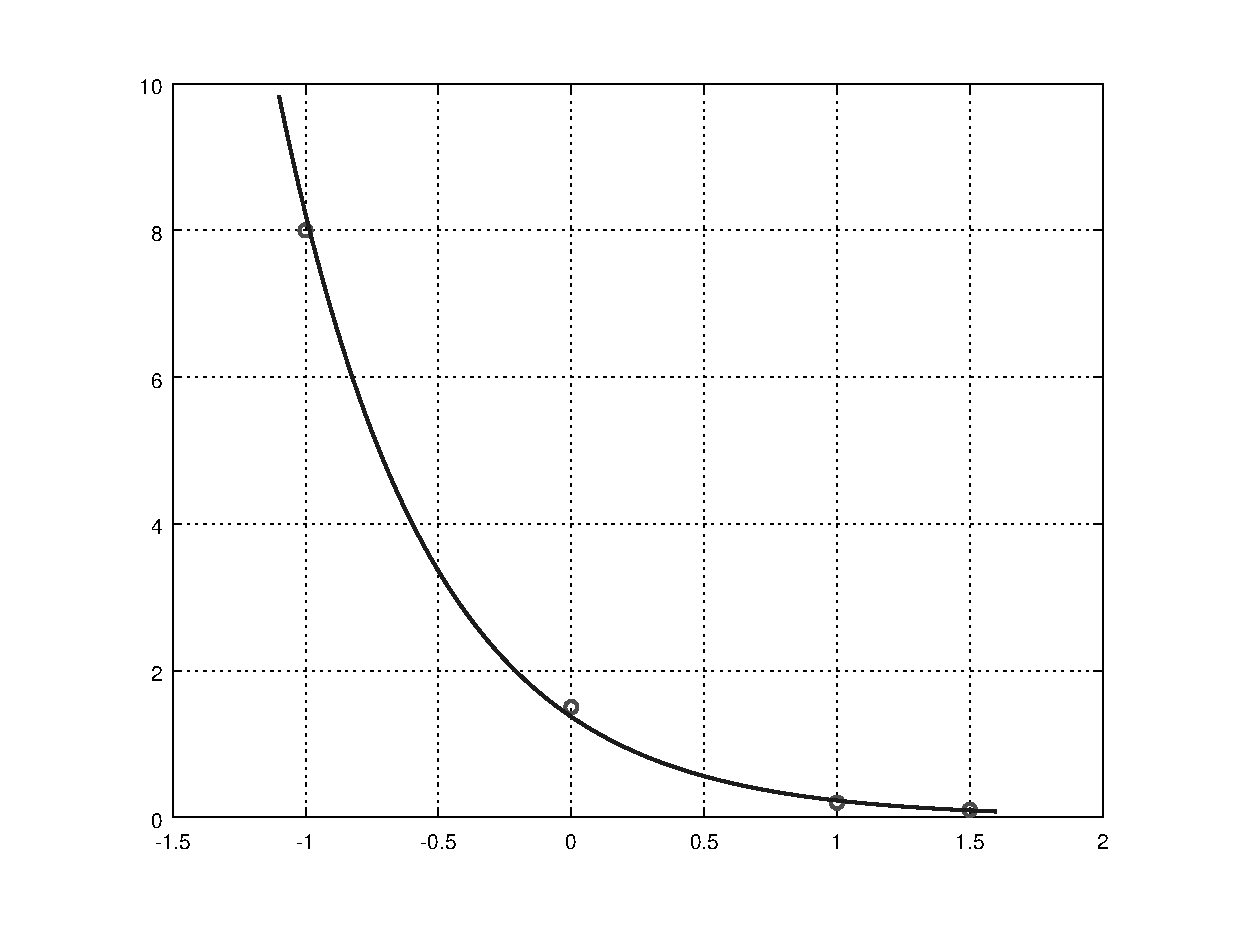
\includegraphics[width=\textwidth]{cap_ajuste/dados/ex_mq_nlin0/ex_mq_nlin0}
  \caption{Esboço da curva ajustada no Exemplo~\ref{ex:mq_nlin0}.}
  \label{fig:ex_mq_nlin0}
\end{figure}

\ifisoctave
O ajuste e um esboço da função ajustada podem ser feitos no \verb+GNU Octave+ com o seguinte código:
\begin{verbatim}
#pontos
x = [-1 0 1 1.5]';
y = [8.0 1.5 0.2 0.1]';

#resol. as eqs. normais
A = [ones(4,1) x];
d = inv(A'*A)*A'*log(y)

#fun. ajustada
c = [exp(d(1)); d(2)]
f = @(x) c(1)*exp(c(2)*x);

#esboco da fun. ajustada
xx = linspace(-1.1,1.6);
plot(x,y,'ro','linewidth',1.5,...
     xx,f(xx),'b-','linewidth',1.5);grid
\end{verbatim}
\fi

\end{ex}

\subsection*{Exercícios}

\begin{exer}\label{exer:mq_reta}
  Determine a reta $y = c_1x + c_2$ que melhor se ajusta, no sentido de mínimos quadrados, aos pontos
  \begin{center}
    \begin{tabular}{l|ccccc}
      $i$ & $1$ & $2$ & $3$ & $4$ & $5$ \\\hline
      $x_i$ & $-2,5$ & $-1,3$ & $0,2$ & $1,7$ & $2,3$\\
      $y_i$ & $3,8$ & $1,5$ & $-0,7$ & $-1,5$ & $-3,2$\\\hline
    \end{tabular}
  \end{center}
Por fim, compute a norma $L^2$ do resíduo, i.e. $\|r(c)\|_2 = \|y - (c_1x - c_2)\|_2$ para os pontos dados.
\end{exer}
\begin{resp}
  \ifisoctave 
  \href{https://github.com/phkonzen/notas/blob/master/src/MatematicaNumerica/cap_ajuste/dados/exer_mq_reta/exer_mq_reta.m}{Código.} 
  \fi
  $c_1 = -1,3259$, $c_2 = 8,66071\E-2$, $\|r(c)\|_2 = 1,01390$.
\end{resp}

\begin{exer}\label{exer:mq_poli}
  Determine o polinômio $y = c_1x^3 + c_2x^2 + c_3x + c_4$ que melhor se ajusta, no sentido de mínimos quadrados, aos pontos
  \begin{center}
    \begin{tabular}{l|ccccc}
      $i$ & $1$ & $2$ & $3$ & $4$ & $5$ \\\hline
      $x_i$ & $-2,5$ & $-1,3$ & $0,2$ & $1,7$ & $2,3$\\
      $y_i$ & $3,8$ & $0,5$ & $2,7$ & $1,2$ & $-1,3$\\\hline
    \end{tabular}
  \end{center}
Por fim, compute a norma $L^2$ do resíduo, i.e. $\|r(c)\|_2$.
\end{exer}
\begin{resp}
  \ifisoctave 
  \href{https://github.com/phkonzen/notas/blob/master/src/MatematicaNumerica/cap_ajuste/dados/exer_mq_poli/exer_mq_poli.m}{Código.} 
  \fi
  $c_1 = -4,50361\E-1$, $c_2 = -2,78350\E-1$, $c_3 = 1,46291$, $c_4 = 2,09648$, $\|r(c)\|_2 = 5,71346$
\end{resp}

\begin{exer}\label{exer:mq_curva}
  Determine a curva $y = c_1\sen x + c_2\cos x + c_3$ que melhor se ajusta, no sentido de mínimos quadrados, aos pontos
  \begin{center}
    \begin{tabular}{l|ccccc}
      $i$ & $1$ & $2$ & $3$ & $4$ & $5$ \\\hline
      $x_i$ & $-2,5$ & $-1,3$ & $0,2$ & $1,7$ & $2,3$\\
      $y_i$ & $3,8$ & $0,5$ & $2,7$ & $1,2$ & $-1,3$\\\hline
    \end{tabular}
  \end{center}
Por fim, compute a norma $L^2$ do resíduo, i.e. $\|r(c)\|_2$.
\end{exer}
\begin{resp}
  \ifisoctave 
  \href{https://github.com/phkonzen/notas/blob/master/src/MatematicaNumerica/cap_ajuste/dados/exer_mq_curva/exer_mq_curva.m}{Código.} 
  \fi
  $c_1 = -2,76842$, $c_2 = -7,17935\E-1$, $c_3 = 1,37014\E-1$, $\|r(c)\|_2 = 2,48880\E+1$
\end{resp}

\begin{exer}\label{exer:mq_nlin0}
  Use a transformação $z = \ln y$ para ajustar, no sentido de mínimos quadrados, a curva $y = c_1e^{c_2(x-c_3)^2}$ aos pontos
  \begin{center}
    \begin{tabular}{l|cccccc}
      $i$ & $1$ & $2$ & $3$ & $4$ & $5$ & $6$ \\\hline
      $x_i$ & $-0,5$ & $0,5$ & $1,3$ & $2,1$ & $2,7$ & $3,1$ \\
      $y_i$ & $0,1$ & $1,2$ & $2,7$ & $0,9$ & $0,2$ & $0,1$ \\\hline
    \end{tabular}
  \end{center}
\end{exer}
\begin{resp}
  \ifisoctave 
  \href{https://github.com/phkonzen/notas/blob/master/src/MatematicaNumerica/cap_ajuste/dados/exer_mq_nlin0/exer_mq_nlin0.m}{Código.} 
  \fi
  $c_1 = 2,10131\E+0$, $c_2 = -9,73859\E-1$, $c_3 = 1.25521\E+0$
\end{resp}
   
\section{Problemas não lineares}\label{cap_ajuste_sec_prob_nlin}

Um problema não linear de mínimos quadrados consiste em ajustar uma dada função $f(x;c)$ que dependa não linearmente dos parâmetros $c = (c_1, c_2, \dotsc, c_m)$, $m\geq 1$, a um dado conjunto de $n\geq m$ pontos $\{(x_i, y_i)\}_{i=1}^n$. Mais especificamente, buscamos resolver o seguinte problema de minimização
\begin{equation}\label{eq:prob_nlin_mq}
  \min_{\{c_1, c_2, \dotsc, c_m\}} \left[E := \sum_{i=1}^n \left(y_i - f(x_i;c)\right)^2\right].
\end{equation}
Aqui, denotaremos por $r(c) := (r_1(c), r_2(c), \dotsc, r_n(c))$ o vetor dos resíduos $r_i(c) := y_i - f(x_i,c)$. Com isso, o problema se resume a encontrar o vetor de parâmetros $c$ que minimiza
\begin{equation}
  E = \|r(c)\|_2^2.
\end{equation}
Tais parâmetros são solução do seguinte sistema de equações
\begin{equation}
  \frac{\p E}{\p c_j} = 2\sum_{i=1}^n r_i(c)\frac{\p}{\p c_j}r_i(c) = 0
\end{equation}
ou, equivalentemente, da equação
\begin{equation}\label{eq:grad_E}
  \nabla E = 0 \Leftrightarrow J_R^T(c)r(c) = 0,
\end{equation}
onde
\begin{equation}
  J_R(c) :=
  \begin{bmatrix}
    \frac{\p r_1}{\p c_1} & \frac{\p r_1}{\p c_2} & \cdots & \frac{\p r_1}{\p c_m}\\
    \frac{\p r_2}{\p c_1} & \frac{\p r_2}{\p c_2} & \cdots & \frac{\p r_2}{\p c_m}\\
    \vdots  & \vdots & \vdots & \vdots \\
    \frac{\p r_n}{\p c_1} & \frac{\p r_n}{\p c_2} & \cdots & \frac{\p r_n}{\p c_m}
  \end{bmatrix}
\end{equation}
é a jacobiana do resíduo $r$ em relação aos parâmetros $c$.

Podemos usar o método de Newton para resolver~\eqref{eq:grad_E}. Para tanto, escolhemos uma aproximação inicial para $c^{(1)} = (c_1^{(1)}, c_2^{(1)}, \dotsc, c_m^{(1)})$ e iteramos
\begin{align}
  H_R(c^{(k)})\delta^{(k)} &= -J_R^T(c)r(c) \label{eq:mqnl_newton1}\\
  c^{(k+1)} &= c^{(k)} + \delta^{(k)} \label{eq:mqnl_newton2},
\end{align}
onde $\delta^{(k)} = (\delta_1^{(k)}, \delta_2^{(k)}, \delta_m^{(k)})$ é a atualização de Newton (ou direção de busca) e $H_R(c) := [h_{p,q}(c)]_{p,q=1}^{m,m}$ é a matriz hessiana, cujos elementos são
\begin{equation}
  h_{p,q} := \sum_{i=1}^n\left\{\frac{\p r_i}{\p c_q}\frac{\p r_i}{\p c_p} + r_i\frac{\p^2 r_i}{\p c_q\p c_p}\right\}.
\end{equation}

\begin{ex}\label{ex:mqnl_newton}
  Consideremos o problema de ajustar, no sentido de mínimos quadrados, a função
  \begin{equation}
    f(x;c) = c_1e^{c_2x}
  \end{equation}
ao seguinte conjunto de pontos
\begin{center}
  \begin{tabular}{l|rrrr}
    $i$ & $1$ & $2$ & $3$ & $4$ \\\hline
    $x_i$ & $-1$ & $0$ & $1$ & $1,5$\\
    $y_i$ & $8,0$ & $1,5$ & $0,2$ & $0,1$\\\hline
  \end{tabular}
\end{center}

Aqui, vamos utilizar a iteração de Newton para o problema de mínimos quadrados, i.e. a iteração dada em \eqref{eq:mqnl_newton1}-\eqref{eq:mqnl_newton2}. Para tanto, para cada $i=1, 2, 3, 4$, precisamos das seguintes derivadas parciais do resíduo $r_i(c) := y_i - c_1e^{c_2x_i}$:
\begin{align}
  &\frac{\p}{\p c_1}r_i(c) = - e^{c_2x_i},\\
  &\frac{\p}{\p c_2}r_i(c) = - c_1x_ie^{c_2x_i},\\
  &\frac{\p^2}{\p c_1^2}r_i(c) = 0,\\
  &\frac{\p^2}{\p c_1\p c_2}r_i(c) = \frac{\p^2}{\p c_2\p c_1}r_i(c) = - x_ie^{c_2x_i},\\
  &\frac{\p^2}{\p c_2^2}r_i(c) = - c_1x_i^2e^{c_2x_i}.
\end{align}

\begin{figure}[h]
  \centering
  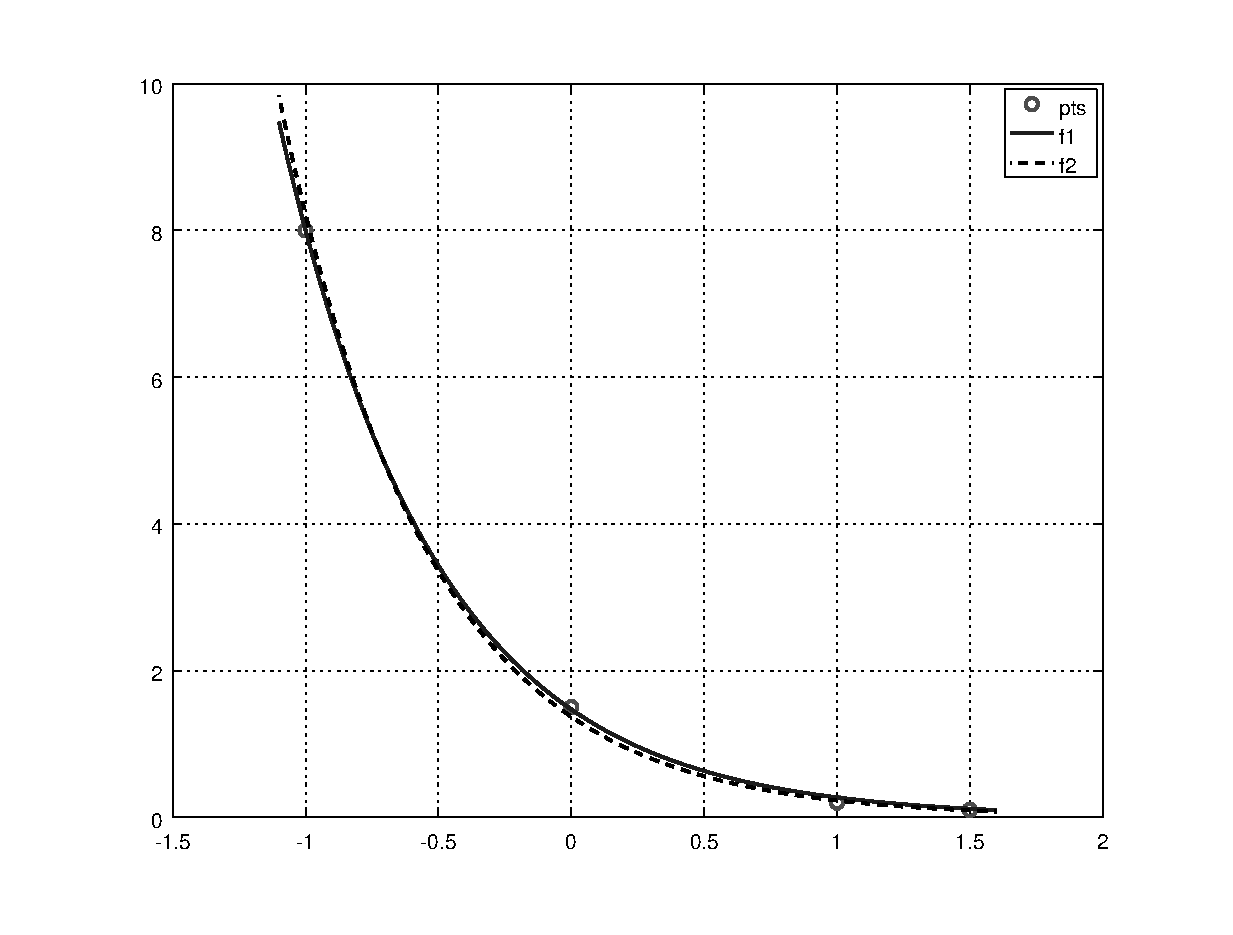
\includegraphics[width=\textwidth]{cap_ajuste/dados/ex_mqnl_N/ex_mqnl_N}
  \caption{Esboço da curva ajustada no Exemplo~\ref{ex:mqnl_newton}.}
  \label{fig:ex_mqnl_newton}
\end{figure}

Com isso e tomando $c^{(1)} = (1,4, ~-1,8)$ (motivado do Exemplo~\ref{ex:mq_nlin0}), computamos as iterações de Newton~\eqref{eq:mqnl_newton1}-\eqref{eq:mqnl_newton2}. Iterando até a precisão de $TOL = 10^{-4}$, obtemos a solução $c_1 = 1,471$ e $c_2 = -1,6938$. Na Figura~\ref{fig:ex_mqnl_newton} vemos uma comparação entre a curva aqui ajustada ($-$) e aquela obtida no Exemplo~\ref{ex:mq_nlin0} ($--$).

\ifisoctave
O ajuste discutido neste exemplo pode ser computado no \verb+GNU Octave+ com o seguinte código:
\begin{verbatim}
#pontos
global x = [-1 0 1 1.5]';
global y = [8.0 1.5 0.2 0.1]';

#fun. objetivo
f = @(x,c) c(1)*exp(c(2)*x);

#residuo
r = @(c) y - f(x,c);

#jacobiana
function A = J(c)
  global x
  A = zeros(4,2);
  A(:,1) = - exp(c(2)*x);
  A(:,2) = - c(1)*x.*exp(c(2)*x);
endfunction

#hessiana
function A = H(c)
  global x
  global y
  A = zeros(2,2);
  A = J(c)'*J(c);
  for i=1:4
    A(1,1) += 0;
    A(1,2) += (y(i) - c(1)*exp(c(2)*x(i))) * ...
              (- x(i)*exp(c(2)*x(i)));
    A(2,1) += (y(i) - c(1)*exp(c(2)*x(i))) * ...
              (- x(i)*exp(c(2)*x(i)));
    A(2,2) += (y(i) - c(1)*exp(c(2)*x(i))) * ...
              (- c(1)*x(i)^2*exp(c(2)*x(i)));
  endfor
endfunction

#aprox. inicial
c = [1.4 -1.8]';

#iteracoes de Newton
k=0;
do
  k+=1;
  delta = - inv(H(c))*J(c)'*r(c);
  c = c + delta;
  [k,c',norm(delta)]
until ((k>10) | (norm(delta)<1e-4))
\end{verbatim}
\fi
\end{ex}

Observamos que a solução obtida no exemplo anterior (Exemplo~\ref{ex:mqnl_newton}) difere da previamente encontrada no Exemplo~\ref{ex:mq_nlin0}. Naquele exemplo, os parâmetros obtidos nos fornecem $E = 6,8\E-2$, enquanto que a solução do exemplo anterior fornece $E = 6,1\E-3$. Isto é esperado, pois naquele exemplo resolvemos um problema aproximado, enquanto no exemplo anterior resolvemos o problema por si.

O emprego do método de Newton para o problema de mínimos quadrados tem a vantagem da taxa de convergência quadrática, entretanto requer a computação das derivadas parciais de segunda ordem do resíduo. Na sequência discutimos alternativas comumente empregadas.

\subsection{Método de Gauss-Newton}

O método de Gauss-Newton é uma técnica iterativa que aproxima o problema não linear de mínimos quadrados \eqref{eq:prob_nlin_mq} por uma sequência de problemas lineares. Para seu desenvolvimento, começamos de uma aproximação inicial $c^{(1)} = (c_1^{(1)}, c_2^{(1)}, \dotsc, c_m^{(1)})$ dos parâmetros que queremos ajustar. Também, assumindo que a $n$-ésima iterada $c^{(k)}$ é conhecida, faremos uso da aproximação de primeira ordem de $f(x,c)$ por polinômio de Taylor, i.e.
\begin{equation}
  f(x;c^{(k+1)}) \approx f(x;c^{(k)}) + \nabla_c f(x;c^{(k)})(c^{(k+1)}-c^{(k)}),
\end{equation}
onde
\begin{equation}
  \nabla_c f(x;c) = \left[\frac{\p}{\p c_1}f(x;c) ~\frac{\p}{\p c_2}f(x;c) ~\cdots ~\frac{\p}{\p c_m}f(x;c)\right].
\end{equation}

O método consiste em obter a solução do problema não linear \eqref{eq:prob_nlin_mq} pelo limite dos seguintes problemas lineares de mínimos quadrados
\begin{align}
  \min_{\delta^{(k)}} &\left[\tilde{E} := \sum_{i=1}^n (y_i - f(x_i,c^{(k)}) - \nabla_c f(x_i;c^{(k)})\delta^{(k)})^2\right] \label{eq:mq_gn0}\\
  &c^{(k+1)} = c^{(k)} + \delta^{(k)}.
\end{align}

Agora, usando a notação de resíduo $r(c) = y - f(x;c)$, observamos que \eqref{eq:mq_gn0} consiste no problema linear de mínimos quadrados
\begin{equation}
  \min_{\delta^{(k)}} \|r(c^{(k)}) + J_R(c^{(k)})\delta^{(k)}\|_2^2,
\end{equation}
o qual é equivalente a resolver as equações normais
\begin{equation}
  J_R^T(c^{(n)})J_R(c^{(n)})\delta^{(n)} = -J_R^T(c)r(c).
\end{equation}

Com isso, dada uma aproximação inicial $c^{(1)}$, a \emph{iteração do método de Gauss-Newton} consiste em
\begin{align}
  &J_R^T(c^{(k)})J_R(c^{(k)})\delta^{(k)} = -J_R^T(c)r(c)\\
  &c^{(k+1)} = c^{(k)} + \delta^{(k)}.
\end{align}

\begin{ex}
  A aplicação da iteração de Gauss-Newton ao problema de mínimos quadrados discutido no Exemplo~\ref{ex:mqnl_newton} nos fornece a mesma solução obtida naquele exemplo (preservadas a aproximação inicial e a tolerância de precisão).

\ifisoctave
A implementação do método de Gauss-Newton para este problema no \verb+GNU Octave+ pode ser feita com o seguinte código:
\begin{verbatim}
#pontos
global x = [-1 0 1 1.5]';
y = [8.0 1.5 0.2 0.1]';

#fun. objetivo
f = @(x,c) c(1)*exp(c(2)*x);

#residuo
r = @(c) y - f(x,c);

#jacobiana
function A = J(c)
  global x
  A = zeros(4,2);
  A(:,1) = - exp(c(2)*x);
  A(:,2) = - c(1)*x.*exp(c(2)*x);
endfunction

#aprox. inicial
c = [1.4 -1.8]';

#iteracoes de Gauss-Newton
k=0;
do
  k+=1;
  delta = - inv(J(c)'*J(c))*J(c)'*r(c);
  c = c + delta;
  [k,c',norm(delta)]
until ((k>10) | (norm(delta)<1e-4))
\end{verbatim}
\fi
\end{ex}

O método de Gauss-Newton pode ser lentamente convergente para problemas muito não lineares ou com resíduos grandes. Nesse caso, métodos de Gauss-Newton com amortecimento são alternativas robustas~\cite{Bjorck1996a,Nocedal2006a}. Na sequência, introduziremos um destes métodos, conhecido como método de Levenberg-Marquardt.

\subsection{Método de Levenberg-Marquardt}

O método de Levenberg-Marquardt é uma variação do método de Gauss-Newton no qual a direção de busca $\delta^{(n)}$ é obtida da solução do seguinte problema regularizado
\begin{equation} \label{eq:mq_gn0}
  \min_{\delta^{(k)}} \{\|r(c^{(k)}) + J_R(c^{(k)})\delta^{(k)}\|_2^2 + \mu^{(k)}\|\delta^{(k)}\|_2^2\}
\end{equation}
ou, equivalentemente,
\begin{equation} \label{eq:mq_gn0}
  \min_{\delta^{(k)}} \left\|
    \begin{bmatrix}
      r(c^{(k)})\\
      0
    \end{bmatrix} +
    \begin{bmatrix}
      J_R(c^{(k)})\\
      \mu^{(k)}I
    \end{bmatrix}
    \delta^{(k)}\right\|_2^2
\end{equation}

A taxa de convergência das iterações de Levenberg-Marquardt é sensível a escolha do parâmetro $\mu^{(k)}\geq 0$. Aqui, faremos esta escolha por tentativa e erro. O leitor pode aprofundar-se mais sobre esta questão na literatura especializada (veja, por exemplo, \cite{Bjorck1996a,Nocedal2006a}).

\begin{obs}
  Quando $\mu^{(k)} \equiv 0$ para todo $n$, o método de Levenberg-Marquardt é equivalente ao método de Gauss-Newton.
\end{obs}

\begin{ex}\label{ex:mqnl_LM}
  Consideremos o problema de mínimos quadrados discutido no Exemplo~\ref{ex:mqnl_newton}. O método de Gauss-Newton falha para este problema se escolhermos, por exemplo, $c^{(1)} = (0, 0)$. Isto ocorre pois, para esta escolha de $c^{(1)}$, a jacobiana $J(c^{(1)})$ não tem posto completo. Entretanto, o método de Levenberg-Marquardt com $\mu^{(k)} = 0,1$ é convergente, mesmo para esta escolha de $c^{(1)}$.

\ifisoctave
A implementação no \verb+GNU Octave+ do método de Levenberg-Marquardt (com $\mu^{(k)}=0,1$ constante) para este problema pode ser feita com o seguinte código:
\begin{verbatim}
#pontos
global x = [-1 0 1 1.5]';
y = [8.0 1.5 0.2 0.1]';

#fun. objetivo
f = @(x,c) c(1)*exp(c(2)*x);

#residuo
r = @(c) y - f(x,c);

#jacobiana
function A = JR(c)
  global x;
  A = zeros(4,2);
  A(:,1) = - exp(c(2)*x);
  A(:,2) = - c(1)*x.*exp(c(2)*x);
endfunction

#aprox. inicial
c = [0 0]';

#param. de amortecimento
mu = 0.1;

#iteracoes de Gauss-Newton
k=0;
do
  k+=1;
  JJ = [JR(c);mu*eye(2,2)];
  delta = - inv(JJ'*JJ)*JJ'*[r(c);zeros(2,1)];
  c = c + delta;
  printf("%d %1.1e %1.3e %1.3e\n", k,norm(delta),c')
until ((k>10) | (norm(delta)<1e-4))
\end{verbatim}
\fi
\end{ex}

\subsection*{Exercícios}

\begin{exer}\label{exer:mqnl_GN}
  Use o método de Gauss-Newton para ajustar, no sentido de mínimos quadrados e com precisão de $10^{-4}$, a curva $y = c_1e^{c_2(x-c_3)^2}$ aos pontos
  \begin{center}
    \begin{tabular}{l|cccccc}
      $i$ & $1$ & $2$ & $3$ & $4$ & $5$ & $6$ \\\hline
      $x_i$ & $-0,5$ & $0,5$ & $1,3$ & $2,1$ & $2,7$ & $3,1$ \\
      $y_i$ & $0,1$ & $1,2$ & $2,7$ & $0,9$ & $0,2$ & $0,1$ \\\hline
    \end{tabular}
  \end{center}
Use as condições iniciais:
\begin{enumerate}[a)]
\item $c_1 = 2,1$, $c_2=-1$ e $c_3=1,3$.
\item $c_1=1$, $c_2=-1$ e $c_3=-1$.
\end{enumerate}
\end{exer}
\begin{resp}
  \ifisoctave 
  \href{https://github.com/phkonzen/notas/blob/master/src/MatematicaNumerica/cap_ajuste/dados/exer_mqnl_GN/exer_mqnl_GN.m}{Código.} 
  \fi
  a) $c_1 = 2,69971\E+0$, $c_2 = -1,44723\E+0$, $c_3 = 1.24333\E+0$; b) divergente.
\end{resp}

\begin{exer}
  Resolva o exercício anterior (Exercício~\ref{exer:mqnl_GN}) usando o método de Levenberg-Marquardt com amortecimento constante $\mu=0,2$.
\end{exer}
\begin{resp}
  \ifisoctave 
  \href{https://github.com/phkonzen/notas/blob/master/src/MatematicaNumerica/cap_ajuste/dados/exer_mqnl_LM/exer_mqnl_LM.m}{Código.} 
  \fi
  a)  $c_1 = 2,69971\E+0$, $c_2 = -1,44723\E+0$, $c_3 = 1.24333\E+0$; b) $c_1 = 2,69971\E+0$, $c_2 = -1,44723\E+0$, $c_3 = 1.24333\E+0$
\end{resp}

%Este trabalho está licenciado sob a Licença Atribuição-CompartilhaIgual 4.0 Internacional Creative Commons. Para visualizar uma cópia desta licença, visite http://creativecommons.org/licenses/by-sa/4.0/deed.pt_BR ou mande uma carta para Creative Commons, PO Box 1866, Mountain View, CA 94042, USA.

\chapter{Derivadas}\label{cap_deriv}
\thispagestyle{fancy}

\ifispython
\begin{obs}\normalfont{(Códigos \verb+Python+)}\label{obs:deriv_python}
  Nos códigos \verb+Python+ inseridos ao longo deste capítulos, estaremos assumindo o seguinte preâmbulo:
\begin{verbatim}
%matplotlib inline
from sympy import *
init_printing()
var('x',real=True)
\end{verbatim}
\end{obs}
\fi

\section{Retas tangentes e derivadas}\label{cap_deriv_sec_retg}

Definimos a {\bf reta secante} ao gráfico de uma dada função $f$ pelos pontos $x_0$ e $x_1$, $x_0\neq x_1$, como sendo a reta determinada pela equação
\begin{equation}
  y = \frac{f(x_1)-f(x_0)}{x_1-x_0}(x-x_0)+f(x_0).
\end{equation}
Isto é, é a reta que passa pelos pontos $(x_0,f(x_0))$ e $(x_1,f(x_1))$. Veja a Figura \ref{fig:retsectg}. Observemos que o coeficiente angular da reta secante é
\begin{equation}
  m_{\text{sec}} = \frac{f(x_1)-f(x_0)}{x_1-x_0}.
\end{equation}

\begin{figure}[H]
  \centering
  \includegraphics[width=0.7\textwidth]{./cap_deriv/dados/fig_retsectg/fig_retsectg}
  \caption{Esboços de uma reta secante (verde) e da reta tangente (vermelho) ao gráfico de uma função.}
  \label{fig:retsectg}
\end{figure}

A {\bf reta tangente} ao gráfico de uma função $f$ em $x=x_0$ é a reta que passa pelo ponto $(x_0, f(x_0))$ e tem coeficiente angular
\begin{equation}\label{eq:mtg}
  m_{\text{tg}} = \lim_{x_1\to x_0} \frac{f(x_1)-f(x_0)}{x_1-x_0}.
\end{equation}
Isto é, a reta de equação
\begin{equation}
  y = m_{\text{tg}}(x-x_0)+f(x_0).
\end{equation}
Menos formal, é a reta limite das retas secantes ao gráfico da função pelos pontos $x_0$ e $x_1$, quando $x_1\to x_0$. Veja a Figura \ref{fig:retsectg}.

\begin{obs}
  Fazendo $h = x_1-x_0$, temos que \eqref{eq:mtg} é equivalente a
  \begin{equation}
    m_{\text{tg}} = \lim_{h\to 0} \frac{f(x_0+h)-f(x_0)}{h}.
  \end{equation}
\end{obs}

\begin{ex}
  Seja $f(x)=x^2$ e $x_0 = 1$. O coeficiente angular da reta tangente ao gráfico de $f$ no ponto $x_0$ é
  \begin{align}
    m_{\text{tg}} &= \lim_{h\to 0} \frac{f(x_0+h)-f(x_0)}{h}\\
                  &= \lim_{h\to 0} \frac{(1+h)^2-1}{h}\\
                  &= \lim_{h\to 0} \frac{1+2h+h^2-1}{h}\\
                  &= \lim_{h\to 0} \frac{2+h}{1} = 2.
  \end{align}
  Assim sendo, a reta tangente ao gráfico de $f(x)=x^2$ no ponto $x_0=1$ tem coeficiente angular $m_{\text{tg}} = 2$ e equação
  \begin{equation}
    y = 2(x-1)+1 = 2x-1.
  \end{equation}
  \ifispython
  Com o \verb+SymPy+, podemos obter a reta tangente com os seguintes comandos:
\begin{verbatim}
h = symbols('h',real=True)
f = lambda x: x**2
x0 = 1
# coef. angular
mtg = limit((f(x0+h)-f(x0))/h,h,0)

# reta tangente
mtg*(x-x0)+f(x0)
\end{verbatim}
  \fi
\end{ex}

\subsection{A derivada em um ponto}

A {\bf derivada} de uma função $f$ {\bf em um ponto} $x=x_0$ é denotada por $f'(x_0)$ ou $\displaystyle \frac{\dd f}{\dd x}(x_0)$ e é definida por
\begin{equation}
  f'(x_0) = \frac{\dd f}{\dd x}(x_0) = \lim_{h\to 0} \frac{f(x_0+h)-f(x_0)}{h}.
\end{equation}

\begin{ex}
  Vejamos os seguintes casos:
  \begin{enumerate}[a)]
  \item $f(x) = k$, $k$ constante.
    \begin{align}
      f'(x_0) &= \lim_{h\to 0} \frac{f(x_0+h)-f(x_0)}{h}\\
              &= \lim_{h\to 0} \frac{k-k}{h} = 0.
    \end{align}
  \item $f(x) = x$.
    \begin{align}
      f'(x_0) &= \lim_{h\to 0} \frac{f(x_0+h)-f(x_0)}{h} \\
              &= \lim_{h\to 0} \frac{x_0+h-x_0}{h} = 1.
    \end{align}
  \item $f(x) = \sqrt{x}$, $x_0=1$.
    \begin{align}
      f'(1) &= \lim_{h\to 0} \frac{\sqrt{1+h}-1}{h}\\
            &= \lim_{h\to 0} \frac{\sqrt{1+h}-1}{h}\frac{\sqrt{1+h}+1}{\sqrt{1+h}+1}\\
            &= \lim_{h\to 0} \frac{1+h-1}{h(\sqrt{1+h}+1)} = \frac{1}{2}.
    \end{align}
  \end{enumerate}
\end{ex}

\subsection*{Exercícios}

\emconstrucao

\section{Função derivada}\label{cap_deriv_sec_deriv}

A {\bf derivada} de uma função $f$ em relação à variável $x$ é a função $\displaystyle f' = \frac{\dd f}{\dd x}$ cujo valor em $x$ é
\begin{equation}\label{eq:derivada}
  \lim_{h\to 0} \frac{f(x+h)-f(x)}{h},
\end{equation}
quando este limite existe. Dizemos que $f$ é {\bf derivável} (ou {\bf diferenciável}) em um ponto $x$ de seu domínio, quando o limite dado em \eqref{eq:derivada} existe. Se isso ocorre para todo número real $x$, dizemos que $f$ é derivável em toda parte.

\begin{ex}
  A derivada de $f(x) = x^2$ é
  \begin{align}
    f'(x) &= \lim_{h\to 0} \frac{f(x+h)-f(x)}{h}\\
          &= \lim_{h\to 0} \frac{(x+h)^2 - x^2}{h}\\
          &= \lim_{h\to 0} \frac{x^2+2xh+h^2-x^2}{h}\\
          &= \lim_{h\to 0} 2x+h = 2x.
  \end{align}
  \ifispython
  Com o \verb+SymPy+, podemos usar os seguintes comandos para verificarmos este resultado:
\begin{verbatim}
h = symbols('h',real=True)
f = lambda x: x**2
limit((f(x+h)-f(x))/h,h,0)
\end{verbatim}
  \fi
\end{ex}

\begin{obs}
  A derivada à direita (à esquerda) de uma função $f$ em um ponto $x$ é definida por
  \begin{equation}
    f_{\pm}'(x) = \frac{\dd f}{\dd x^{\pm}} = \lim_{h\to 0^\pm} \frac{f(x+h)-f(x)}{h}.
  \end{equation}
  Desta forma, no caso de pontos extremos do domínio de uma função, empregamos a derivada lateral correspondente.
\end{obs}

\begin{ex}
  A função valor absoluto é derivável para todo $x\neq 0$ e não é derivável em $x=0$. De fato, para $x<0$ temos
  \begin{align}
    f'(x) &= \lim_{x\to 0} \frac{|x+h|-|x|}{h}\\
          &= \lim_{h\to 0} \frac{-(x+h)+x}{h}\\
          &= \lim_{h\to 0} \frac{h}{h} = 1.
  \end{align}
  Analogamente, para $x>0$ temos
  \begin{align}
    f'(x) &= \lim_{x\to 0} \frac{|x+h|-|x|}{h}\\
          &= \lim_{x\to 0} \frac{x+h-x}{h}\\
          &= \lim_{x\to 0} \frac{h}{h} = 1.
  \end{align}
  Agora, para $x=0$, devemos verificar as derivadas laterais:
  \begin{align}
    f'_+(0) &= \lim_{h\to 0^+} \frac{|h|-|0|}{h} = \lim_{h\to 0^+} \frac{h}{h} = 1,\\
    f'_-(0) &= \lim_{h\to 0^-} \frac{|h|-|0|}{h} = \lim_{h\to 0^-} \frac{-h}{h} = -1.
  \end{align}
  Como as derivadas laterais são diferentes, temos que $y = |x|$ não é derivável em $x=0$.
\end{ex}

\begin{ex}
  Vamos calcular a derivada de $f(x) = \sqrt{x}$. Para $x=0$, só faz sentido calcular a derivada lateral à direta:
  \begin{equation}
    f'(0) = \lim_{h\to 0^+} \frac{\sqrt{h}-\sqrt{0}}{h} = +\infty.
  \end{equation}
  Ou seja, $f(x) = \sqrt{x}$ não é derivável em $x=0$. Agora, para $x> 0$, temos
  \begin{align}
    f'(x) &= \lim_{h\to 0} \frac{\sqrt{x+h}-\sqrt{x}}{h}\\
          &= \lim_{h\to 0} \frac{\sqrt{x+h}-\sqrt{x}}{h}\frac{\sqrt{x+h}+\sqrt{x}}{\sqrt{x+h}+\sqrt{x}}\\
          &= \lim_{h\to 0} \frac{x+h-x}{h(\sqrt{x+h}+\sqrt{x})}\\
          &= \frac{1}{2\sqrt{x}}.
  \end{align}
\end{ex}

\subsection*{Exercícios}

\emconstrucao


\section{Regras básicas de derivação}\label{cap_deriv_sec_regras}

Vejamos as derivadas da função constante e da função potência.
\begin{itemize}
\item $\displaystyle \frac{\dd k}{\dd x} = 0$, onde $k$ é uma constante.

  Dem.: Com $f(x) \equiv k$ temos
  \begin{align}
    \frac{\dd k}{\dd x} &= \lim_{h\to 0} \frac{f(x+h)-f(x)}{h}\\
                        &= \lim_{h\to 0} \frac{k-k}{h} \\
                        &= \lim_{h\to 0} 0 = 0.
  \end{align}
  \ifispython
  No \verb+SymPy+, podemos usar os seguintes comandos para obtermos tal regra de derivação:
\begin{verbatim}
k = symbols('k',real=True)
diff(k,x)
\end{verbatim}
  \fi
  

\item $\displaystyle \frac{\dd x^n}{\dd x} = nx^{n-1}$, para $n$ inteiro positivo.

  Dem.: Com $f(x) = x^n$, temos
  \begin{align}
    \frac{\dd x^n}{\dd x} &= \lim_{h\to 0} \frac{f(x+h)-f(x)}{h}\\
                          &= \lim_{h\to 0} \frac{(x+h)^n-x^n}{h} \\
                          &= \lim_{h\to 0} \frac{x^n+nx^{n-1}h+\frac{n(n-1)}{2}x^{n-2}h^2 + \cdots +h^n-x^n}{h}\\
                          &= \lim_{h\to 0} nx^{n-1}+\frac{n(n-1)}{2}x^{n-2}h+\cdots+h^{n-1}\\
                          &= nx^{n-1}.
  \end{align}
  \ifispython
  No \verb+SymPy+, podemos usar os seguintes comandos para obtermos tal regra de derivação:
\begin{verbatim}
n = symbols('n',integer=True, positive=True)
simplify(diff(x**n,x))
\end{verbatim}
  \fi
\end{itemize}

\begin{ex}
  Vejamos os seguintes casos:
  \begin{enumerate}[a)]
  \item $\displaystyle \frac{\dd \sqrt{2}}{\dd x} = 0$.
  \item $\displaystyle \frac{\dd x^3}{\dd x} = 3x^2$.
  \end{enumerate}
\end{ex}

\subsection{Multiplicação por constante e soma}

Sejam $c$ um número real, $u$ e $v$ funções. Temos as seguintes regras básicas de derivação:
\begin{itemize}
\item $\displaystyle (cu)' = cu'$.

  Dem.:
  \begin{align}
    \frac{\dd}{\dd x}(cu)(x) &= \lim_{h\to 0} \frac{cu(x+h)-cu(x)}{h} \\
                          &= c\lim_{h\to 0} \frac{u(x+h)-u(x)}{h} \\
                          &= c\frac{\dd u}{\dd x}.
  \end{align}
  \ifispython
  No \verb+SymPy+, podemos usar os seguintes comandos para obtermos tal regra de derivação:
\begin{verbatim}
c = symbols('c', real=True)
u = Function('u', real=True)(x)
diff(c*u,x)
\end{verbatim}
  \fi

\item $\displaystyle (u\pm v)' = u'\pm v'$.

  Dem.:
  \begin{align}
    (u\pm v)'(x) &= \lim_{h\to 0} \frac{(u\pm v)(x+h)-(u\pm v)(x)}{h}\\
                              &= \lim_{h\to 0} \left[\frac{u(x+h)-u(x)}{h}\pm\frac{v(x+h)-v(x)}{h}\right]\\
              &= u'(x) \pm v'(x).
  \end{align}
  \ifispython
  No \verb+SymPy+, podemos usar os seguintes comandos para obtermos a regra de derivação para soma:
\begin{verbatim}
u = Function('u', real=True)(x)
v = Function('v', real=True)(x)
diff(u+v,x)
\end{verbatim}
  \fi
\end{itemize}

\begin{ex}
  \begin{align}
    \frac{\dd}{\dd x}(x^3-2x -1) &= \frac{\dd}{\dd x}x^3 -2\frac{\dd x}{\dd x} - \frac{\dd 1}{\dd x}\\
                                 &= 3x^2-2.
  \end{align}
\end{ex}

\subsection{Produto e quocientes}

Sejam $y = u(x)$ e $y = v(x)$ funções deriváveis, com $v(x)\neq 0$. Então:
\begin{itemize}
\item $(uv)' = u'v+uv'$.

  Dem.:
  \begin{align}
    (uv)'(x) &= \lim_{h\to 0} \frac{(uv)(x+h)-(uv)(x)}{h}\\
             &= \lim_{h\to 0} \frac{u(x+h)v(x+h)-u(x)v(x)}{h}\\
             &= \lim_{h\to 0} \left[\frac{u(x+h)v(x+h)-u(x)v(x+h)}{h}\right.\\
             &\qquad\quad+ \left.\frac{u(x)v(x+h)-u(x)v(x)}{h}\right]\\
             &= \lim_{h\to 0} \frac{u(x+h)-u(x)}{h}v(v+h) \\
             &+ \lim_{h\to 0} u(x)\frac{v(x+h)-v(x)}{h}\\
             &= u'(x)v(x) + u(x)v'(x).
  \end{align}
  \ifispython
  No \verb+SymPy+, podemos usar os seguintes comandos para obtermos tal regra de derivação:
\begin{verbatim}
u = Function('u', real=True)(x)
v = Function('v', real=True)(x)
diff(u*v,x)
\end{verbatim}
  \fi
\item $\displaystyle\left(\frac{u}{v}\right)' = \frac{u'v-uv'}{v^2}$.

  Dem.:
  \begin{align}
    \left(\frac{u}{v}\right)'(x) &= \lim_{h\to 0} \frac{\left(\frac{u}{v}\right)(x+h)-\left(\frac{u}{v}\right)(x)}{h} \\
                                 &= \lim_{h\to 0} \frac{\frac{u(x+h)v(x)-u(x)v(x+h)}{v(x+h)v(x)}}{h}\\
                                 &= \lim_{h\to 0} \left[\frac{u(x+h)v(x)-u(x)v(x)}{h}\right. \\
                                 &\qquad\quad - \left.\frac{u(x)v(x+h)-u(x)v(x)}{h}\right]\frac{1}{v(x)v(x+h)}\\
                                 &= \left[\lim_{h\to 0} \frac{u(x+h)-u(x)}{h}v(x)\right. \\
                                 &\left. - \lim_{h\to 0} u(x)\frac{v(x+h)-v(x)}{h}\right]\lim_{h\to 0} \frac{1}{v(x)v(x+h)}\\
                                 &= \frac{u'(x)v(x)-u(x)v'(x)}{v^2(x)}.
  \end{align}
  \ifispython
  No \verb+SymPy+, podemos usar os seguintes comandos para obtermos tal regra de derivação:
\begin{verbatim}
u = Function('u', real=True)(x)
v = Function('v', real=True)(x)
simplify(diff(u/v,x))
\end{verbatim}
  \fi
\end{itemize}

\begin{ex}
  Vejamos os seguintes casos:
  \begin{enumerate}[a)]
  \item
    \begin{align}
      \frac{\dd}{\dd x}\left[(x^2+x)(1 + x^3)\right] &= \left[\frac{\dd}{\dd x} (x^2+x)\right](1+x^3) \\
                                                     &+ (x^2+x)\left[\frac{\dd}{\dd x}(1+x^3)\right]\\
                                                     &= (2x+1)(1+x^3)+(x^2+x)3x^2\\
                                                     &= 2x+2x^4+1+x^3+3x^4+3x^3\\
                                                     &= 5x^4+4x^3+2x+1.
    \end{align}
    \ifispython
    Com o \verb+SymPy+, podemos computar esta derivada com o seguinte comando\footnote{Veja a Observação \ref{obs:deriv_python}.}:
\begin{verbatim}
d = diff((x**2+x)*(1+x**3),x)
simplify(d)
\end{verbatim}
    \fi

\item
  \begin{align}
    \frac{\dd}{\dd x}\left(\frac{x^2+x}{1-x^3}\right) &= \frac{\left[\frac{\dd}{\dd x}(x^2+x)\right](1-x^3)-(x^2+x)\left[\frac{\dd}{\dd x}(1-x^3)\right]}{(1-x^3)^2}\\
                                                      &= \frac{(2x+1)(1-x^3)+(x^2+x)3x^2}{1-2x^3+x^6} \\
                                                      &= \frac{2x-2x^4+1-x^3+3x^4+3x^3}{1-2x^3+x^6} \\
                                                      &= \frac{x^4+2x^3+2x+1}{x^6-2x^3+1}
  \end{align}
  \ifispython
  Com o \verb+SymPy+, podemos computar esta derivada com o seguinte comando\footnote{Veja a Observação \ref{obs:deriv_python}.}:
\begin{verbatim}
d = diff((x**2+x)/(1-x**3),x)
simplify(d)
\end{verbatim}
  \fi
  \end{enumerate}
\end{ex}

\begin{obs}\normalfont{(Derivada de funções potência)}
  No início desta seção, vimos que
  \begin{equation}
    \frac{\dd x^n}{\dd x} = nx^{n-1},
  \end{equation}
  para $n>0$ inteiro. Agora, podemos afirmar que este é, também, o caso quando $n<0$ inteiro. De fato, se $n < 0$, então
  \begin{align}
    (x^n)' &= \left(\frac{1}{x^{-n}}\right)\\
           &= \frac{(1)'x^{-n}-1\cdot\left(x^{-n}\right)'}{\left(x^{-n}\right)^2}\\
           &= \frac{0-(-n)x^{-n-1}}{x^{-2n}}\\
           &= nx^{2n-n-1} = nx^{n-1}.
  \end{align}
  \ifispython
  O \verb+SymPy+, obtém o mesmo resultado, verifique usando os comandos:
\begin{verbatim}
var('n',integer=True)
simplify(diff(x**n,x))
\end{verbatim}
  \fi
\end{obs}

\begin{ex}
  \begin{equation}
    \frac{\dd}{\dd x}x^{-5} = -5x^{-5-1} = -5x^{-4}.
  \end{equation}
\end{ex}


\subsection{Derivadas de funções exponenciais}

Seja $f(x) = a^x$, $a>0$ e $a\neq 1$. Então
\begin{align}
  f'(x) &= \lim_{h\to 0} \frac{f(x+h)-f(x)}{h}\\
        &= \lim_{h\to 0} \frac{a^{x+h}-a^x}{h} \\
        &= \lim_{h\to 0} \frac{a^xa^h-a^x}{h} \\
        &= a^x \lim_{h\to 0} \frac{a^h-1}{h}
\end{align}
Pode-se mostrar que
\begin{equation}
  \lim_{h\to 0} \frac{a^h-1}{h} = \ln a.
\end{equation}
Desta forma, temos
\begin{equation}
  \frac{\dd a^x}{\dd x} = a^x\ln a.
\end{equation}

Para a função exponencial natural $y = e^x$, temos
\begin{align}
  \frac{\dd e^x}{\dd x} &= e^x\ln e\\
                        &= e^x.
\end{align}

\begin{ex}
  
\end{ex}

\emconstrucao

\subsection*{Exercícios}

\emconstrucao

\section{Aplicações}\label{cap_deriv_sec_apl}

Observamos que a razão
\begin{equation}
  \frac{f(x_0+h)-f(x_0)}{h}
\end{equation}
pode ser entendida como a {\bf taxa de variação média} de $f$ no intervalo de $x_0$ a $x_0+h$, $h\neq 0$. Tomando o limite de $h\to 0$,
\begin{equation}
  \lim_{h\to 0} \frac{f(x_0+h)-f(x_0)}{h} = f'(x_0),
\end{equation}
temos a {\bf taxa de variação instantânea} de $f$ em relação a $x$ no ponto $x_0$, i.e. a taxa com que $f$ varia no ponto $x=x_0$.

\begin{ex}
  Suponhemos que o número de litros de água em um tanque, $t$ minutos depois de iniciar seu esvaziamento, é dado por $V = 2000(40-t)^2$. Deste modelo, podemos tirar várias conclusões.
  \begin{enumerate}[a)]
  \item A taxa média do volume de água no tanque nos primeiros $10$ minutos é:
    \begin{align}
      \frac{V(t_0+h}-V(t_0){h} &= \frac{V(0+10)-V(0)}{10} \\
                               &= \frac{2000\cdot 30^2-2000\cdot 40^2}{10} \\
                               &= 200(900-1600) = 100\,000 ~ \text{L}/\text{min}.
    \end{align}
  \item Podemos obter a taxa instantânea do volume de áqua no tanque em $t=10$ minutos. Para tanto, calculamos a derivada
    \begin{align}
      V'(t) &= -160\,000 + 4000t. 
    \end{align}
    Assim, temos que a taxa de variação instantânea do volume de água no tanque em $t=10$ minutos é:
    \begin{equation}
      V'(10) = 160\,000+40\,000 = 120\,000 ~\text{L}/\text{min}.
    \end{equation}
  \end{enumerate}
\end{ex}

\emconstrucao

\subsection*{Exercícios}

\emconstrucao
%Este trabalho está licenciado sob a Licença Atribuição-CompartilhaIgual 4.0 Internacional Creative Commons. Para visualizar uma cópia desta licença, visite http://creativecommons.org/licenses/by-sa/4.0/deed.pt_BR ou mande uma carta para Creative Commons, PO Box 1866, Mountain View, CA 94042, USA.

\chapter{Técnicas de extrapolação}\label{cap_extrapl}
\thispagestyle{fancy}

Neste capítulo, estudamos algumas técnicas de extrapolação, as quais serão usadas nos próximos capítulos.

\section{Extrapolação de Richardson}\label{cap_extrapl_sec_Richardson}

Seja $F_1(h)$ uma aproximação de $I$ tal que
\begin{equation}\label{eq:extrapl_aux1}
  I = F_1(h) + \underbrace{k_1h + k_2h^2 + k_3h^3 + O(h^4)}_{\text{erro de truncamento}}.
\end{equation}
Então, dividindo $h$ por $2$, obtemos
\begin{equation}\label{eq:extrapl_aux2}
  I = F_1\left(\frac{h}{2}\right) + k_1\frac{h}{2} + k_2\frac{h^2}{4} + k_3\frac{h^3}{8} + O(h^4).
\end{equation}
Agora, de forma a eliminarmos o termo de ordem $h$ das expressões acima, subtraímos \eqref{eq:extrapl_aux1} de $2$ vezes~\eqref{eq:extrapl_aux2}, o que nos leva a
\begin{equation}\label{eq:extrapl_aux3}
  I = \underbrace{\left[F_1\left(\frac{h}{2}\right) + \left(F_1\left(\frac{h}{2}\right) - F_1(h)\right)\right]}_{F_2(h)} - k_2\frac{h^2}{2} - k_3\frac{3h^3}{4} + O(h^4).
\end{equation}
Ou seja, denotando
\begin{equation}
  F_2(h) := F_1\left(\frac{h}{2}\right) + \left(F_1\left(\frac{h}{2}\right) - F_1(h)\right)
\end{equation}
temos que $N_2(h)$ é uma aproximação de $I$ com erro de truncamento da ordem de $h^2$, uma ordem a mais de $N_1(h)$. Ou seja, esta combinação de aproximações de ordem de truncamento $h$ nos fornece uma aproximação de ordem de truncamento $h^2$.

Analogamente, consideremos a aproximação de $I$ por $N_2(h/2), i.e.$
\begin{equation}\label{eq:extrapl_aux4}
  I = F_2\left(\frac{h}{2}\right) - k_2\frac{h^2}{8} - k_2\frac{3h^3}{32} + O(h^4)
\end{equation}
Então, subtraindo~\eqref{eq:extrapl_aux3} de $4$ vezes~\eqref{eq:extrapl_aux4} de, obtemos
\begin{equation}\label{eq:extrapl_aux5}
  I = \underbrace{\left[3F_2\left(\frac{h}{2}\right) + \left(F_2\left(\frac{h}{2}\right) - F_2(h)\right)\right]}_{F_3(h)} + k_3\frac{3h^3}{8} + O(h^4).
\end{equation}
Observemos, ainda, que $N_3(h)$ pode ser reescrita na forma
\begin{equation}
  F_3(h) = F_2\left(\frac{h}{2}\right) + \frac{F_2\left(\frac{h}{2}\right) - F_2(h)}{3},
\end{equation}
a qual é uma aproximação de ordem $h^3$ para $I$.

Para fazermos mais um passo, consideramos a aproximação de $I$ por $F_3(h/2)$, i.e.
\begin{equation}\label{eq:extrapl_aux6}
  I = F_3\left(\frac{h}{2}\right) + k_3\frac{3h^3}{64} + O(h^4).
\end{equation}
E, então, subtraindo~\eqref{eq:extrapl_aux5} de $8$ vezes~\eqref{eq:extrapl_aux6}, temos
\begin{equation}
  I = \underbrace{\left[F_3\left(\frac{h}{2} \right)+ \left(\frac{F_3\left(\frac{h}{2}\right)-F_3(h)}{7}\right)\right]}_{F_4(h)} + O(h^4).
\end{equation}
Ou seja,
\begin{equation}
  F_4(h) = \left[F_3\left(\frac{h}{2}\right) + \frac{F_3\left(\frac{h}{2}\right)-F_3(h)}{7}\right]
\end{equation}
é uma aproximação de $I$ com erro de truncamento da ordem $h^4$. Estes cálculos nos motivam o seguinte teorema.

\begin{teo}\label{teo:Richardson}
  Seja $F_1(h)$ uma aproximação de $I$ com erro de truncamento da forma
  \begin{equation}
    I-F_1(h) = \sum_{i=1}^n k_1h^i + O(h^{n+1}).
  \end{equation}
Então, para $j\geq 2$,
\begin{equation}
  F_j(h) := F_{j-1}\left(\frac{h}{2}\right) + \frac{F_{j-1}\left(\frac{h}{2}\right) - F_{j-1}(h)}{2^{j-1}-1}
\end{equation}
é uma aproximação de $I$ com erro de truncamento da forma
\begin{align}
  I-F_{j}(h) &= \sum_{i=j}^n (-1)^{j-1}\frac{\left(2^{i-1}-1\right)\prod_{l=1}^{j-2}\left(2^{i-l-1}-1\right)}{2^{(j-1)(i-j+1)}d_j}k_ih^i \nonumber \\
           & + O(h^{n+1}),
\end{align}
onde $d_{j}$ é dado recursivamente por $d_{j+1}=2^{j-1}d_j$, com $d_2=1$.
\end{teo}
\begin{dem}
  Fazemos a demonstração por indução. O resultado para $j=2$ segue de~\eqref{eq:extrapl_aux3}. Assumimos, agora, que vale
  \begin{align}
    I-F_{j}(h) &= (-1)^{j-1}\frac{\left(2^{j-1}-1\right)\prod_{l=1}^{j-2}\left(2^{j-l-1}-1\right)}{2^{(j-1)}d_j}k_jh^j \nonumber \\
              &+ \sum_{i=j+1}^n (-1)^{j-1}\frac{\left(2^{i-1}-1\right)\prod_{l=1}^{j-2}\left(2^{i-l-1}-1\right)}{2^{(j-1)(i-j+1)}d_j}k_ih^i \nonumber \\
              & + O(h^{n+1}).\label{eq:extrapl_aux7}
  \end{align}
para $j\geq 2$. Então, tomamos
\begin{align}
  I-F_{j}\left(\frac{h}{2}\right) &= (-1)^{j-1}\frac{\left(2^{j-1}-1\right)\prod_{l=1}^{j-2}\left(2^{j-l-1}-1\right)}{2^{(j-1)}d_j}k_j\frac{h^j}{2^j} \nonumber \\
              &+ \sum_{i=j+1}^n (-1)^{j-1}\frac{\left(2^{i-1}-1\right)\prod_{l=1}^{j-2}\left(2^{i-l-1}-1\right)}{2^{(j-1)(i-j+1)}d_j}k_i\frac{h^i}{2^i} \nonumber \\
              & + O(h^{n+1}). \label{eq:extrapl_aux8}
\end{align}
Agora, subtraímos~\eqref{eq:extrapl_aux7} de $2^{j}$ vezes~\eqref{eq:extrapl_aux8}, o que nos fornece
\begin{align}
  I &= \left[F_{j}\left(\frac{h}{2}\right) + \frac{F_{j}\left(\frac{h}{2}\right) - F_{j}(h)}{2^{j}-1}\right] \nonumber\\
    &+ \sum_{i=j+1}^n (-1)^{(j+1)-1}\frac{\left(2^{i-1}-1\right)\prod_{l=1}^{(j+1)-2}\left(2^{i-l-1}-1\right)}{2^{((j+1)-1)(i-(j+1)+1)}2^{j-1}d_j}k_ih^i\nonumber \\
              & + O(h^{n+1}).
\end{align}
\end{dem}

\begin{corol}
  Seja $F_1(h)$ uma aproximação de $I$ com erro de truncamento da forma
  \begin{equation}
    I-F_1(h) = \sum_{i=1}^n k_1h^{2i} + O(h^{2n+2}).
  \end{equation}
Então, para $j\geq 2$,
\begin{equation}
  F_j(h) := F_{j-1}\left(\frac{h}{2}\right) + \frac{F_{j-1}\left(\frac{h}{2}\right) - F_{j-1}(h)}{4^{j-1}-1}
\end{equation}
é uma aproximação de $I$ com erro de truncamento da forma
\begin{align}
  I-F_{j}(h) &= \sum_{i=j}^n (-1)^{j-1}\frac{\left(4^{i-1}-1\right)\prod_{l=1}^{j-2}\left(4^{i-l-1}-1\right)}{4^{(j-1)(i-j+1)}d_j}k_ih^{2i} \nonumber \\
           & + O(h^{n+1}),
\end{align}
onde $d_{j}$ é dado recursivamente por $d_{j+1}=4^{j-1}d_j$, com $d_2=1$.
\end{corol}
\begin{dem}
  A demonstração é análoga ao do Teorema~\ref{teo:Richardson}.
\end{dem}

\begin{ex}
  Dada uma função $f(x)$, consideremos sua aproximação por diferenças finitas progressiva de ordem $h$, i.e.
  \begin{align}
    \underbrace{f'(x)}{I} &= \underbrace{\frac{f(x+h)-f(x)}{h}}_{F_1(h)}\nonumber\\
    &+ \frac{f''(x)}{2}h + \frac{f'''(x)}{6}h^2 + O(h^3).
  \end{align}
Estão, considerando a primeira extrapolação de Richardson, temos
\begin{align}
  F_2(h) &= F_1\left(\frac{h}{2}\right) + \left(F_1\left(\frac{h}{2}\right) - F_1(h)\right)\\
  &= 4\frac{f(x+h/2)-f(x)}{h} - \frac{f(x+h)-f(x)}{h}\\
  &= \frac{-f(x+h)+4f(x+h/2)-3f(x)}{h},
\end{align}
a qual é a fórmula de diferenças finitas progressiva de três pontos com passo $h/2$, i.e. $D_{+,(h/2)^2}f(x)$ (veja, Fórmula~\eqref{eq:dfp_3pts}).
\end{ex}

\begin{ex}
  Dada uma função $f(x)$, consideremos sua aproximação por diferenças finitas central de ordem $h^2$, i.e.
  \begin{align}
    \underbrace{f'(x)}{I} &= \underbrace{\frac{f(x+h)-f(x-h)}{2h}}_{F_1(h)} \nonumber \\
                          &- \frac{f'''}{6}h^2 - \frac{f^{(5)}(x)}{120}h^4 + O(h^6).
  \end{align}
Estão, considerando a primeira extrapolação de Richardson, temos
\begin{align}
  F_2(h) &= F_1\left(\frac{h}{2}\right) + \frac{\left(F_1\left(\frac{h}{2}\right) - F_1(h)\right)}{3}\\
  &= \frac{1}{6h}\left[f(x-h)-8f(x-h/2)+8f(x+h/2)-f(x+h)\right]
\end{align}
a qual é a fórmula de diferenças finitas central de cinco pontos com passo $h/2$, i.e. $D_{+,(h/2)^4}f(x)$ (veja, Fórmula~\eqref{eq:dfc_5pts}).
\end{ex}

\subsection{Sucessivas extrapolações}

Sucessivas extrapolações de Richardson podem ser computadas de forma robusta com o auxílio de uma tabela. Seja $F_1(h)$ uma dada aproximação de uma quantidade de interesse $I$ com erro de truncamento da forma
\begin{equation}
  I-F_1(h) = k_1h + k_2h^2 + k_3h^3 + \cdots + k_nh^n + O(h^{n+1}).
\end{equation}
Então, as sucessivas extrapolações $F_2(h)$, $F_3(h)$, $\dotsc$, $F_n(h)$ podem ser organizadas na seguinte forma tabular
\begin{equation}
  T = \left[\begin{array}{lllll}
    F_1(h)\\
    F_1(h/2) & F_2(h) \\
    F_1(h/2^2) & F_2(h/2) & F_3(h) \\
    \vdots & \vdots & \vdots \\
    F_1(h/2^n) & F_2(h/2^{n-1}) & F_3(h/2^{n-2}) & \cdots & F_n(h)
  \end{array}\right]
\end{equation}
Desta forma, temos que
\begin{equation}
  F_j\left(\frac{h}{2^{i-1}}\right) = t_{i,j-1} + \frac{t_{i,j-1}-t_{i-1,j-1}}{2^{j-1}-1}
\end{equation}
com $j=2, 3, \dotsc, n$ e $j\geq i$, onde $t_{i,j}$ é o elemento da $i$-ésima linha e $j$-ésima coluna da matriz $T$.

\begin{ex}\label{ex:Richardson_suc_h}
  Consideremos o problema de aproximar a derivada da função $f(x) = \sen(x)$ no ponto $\pi/3$. Usando a fórmula de diferenças finitas progressiva de ordem $h$ obtemos
  \begin{align}
    f'\left(\frac{\pi}{3}\right) &= \underbrace{\frac{f\left(\frac{\pi}{3}+h\right)-f\left(\frac{\pi}{3}\right)}{h}}_{F_1(h) := D_{+,h}f(\pi/3)} \nonumber\\
          &+ \frac{f''(x)}{2}h + \frac{f'''(x)}{6}h^2 + \cdots \label{eq:ex_Richardson_suc_h}
  \end{align}
Na Tabela~\ref{tab:ex_Richardson_suc_h} temos os valores das aproximações de $f'(\pi/3)$ computadas via sucessivas extrapolações de Richardson a partir de \eqref{eq:ex_Richardson_suc_h} com $h=0.1$.

\begin{table}[h!]
  \centering
  \caption{Resultados referente ao Exemplo~\ref{ex:Richardson_suc_h}.}
  \begin{tabular}{cccc}\hline
    $O(h)$ & $O(h^2)$ & $O(h^3)$ & $O(h^4)$\\ \hline
    $4,55902\E-1$ \\
    $4,78146\E-1$ & $5,00389\E-1$ \\
    $4,89123\E-1$ & $5,00101\E-1$ & $5,00005\E-1$ \\
    $4,94574\E-1$ & $5,00026\E-1$ & $5,00001\E-1$ & $5,00000\E-1$ \\\hline
  \end{tabular}
  \label{tab:ex_Richardson_suc_h}
\end{table}

No \verb+GNU Octave+, podemos fazer estes cálculos com o seguinte código:
\begin{verbatim}
#funcao
f = @(x) sin(x);
x=pi/3;

#aproximacao de ordem 1
dfp = @(x,h) (f(x+h)-f(x))/h;
h=0.1;

#tabela c/ sucessivas extrapolacoes
T=zeros(4,4);
for i=1:4
  T(i,1) = dfp(x,h/2^(i-1));
endfor
for j=2:4
  for i=j:4
    T(i,j) = T(i,j-1) ... 
           + (T(i,j-1)-T(i-1,j-1))/(2^(j-1)-1);
  endfor
endfor
\end{verbatim}
\end{ex}

\begin{ex}\label{ex:Richardson_suc_h2}
  Novamente, consideremos o problema de aproximar a derivada da função $f(x) = \sen(x)$ no ponto $\pi/3$. A fórmula de diferenças finitas central de ordem $h^2$ tem a forma
  \begin{align}
    f'\left(\frac{\pi}{3}\right) &= \underbrace{\frac{f\left(\frac{\pi}{3}+h\right)-f\left(\frac{\pi}{3}-h\right)}{2h}}_{F_1(h) := D_{0,h^2}f(\pi/3)} \nonumber\\
          &- \frac{f'''(x)}{6}h^2 + \frac{f^{(5)}(x)}{120}h^4 - \cdots \label{eq:ex_Richardson_suc_h2}
  \end{align}
Na Tabela~\ref{tab:ex_Richardson_suc_h2} temos os valores das aproximações de $f'(\pi/3)$ computadas via sucessivas extrapolações de Richardson a partir de \eqref{eq:ex_Richardson_suc_h2} com $h=1$.

\begin{table}[h!]
  \centering
  \caption{Resultados referente ao Exemplo~\ref{ex:Richardson_suc_h2}.}
  \begin{tabular}{cccc}\hline
    $O(h^2)$ & $O(h^4)$ & $O(h^6)$ & $O(h^8)$\\ \hline
    $4,20735\E-1$ \\
    $4,79426\E-1$ & $4,98989\E-1$ \\
    $4,94808\E-1$ & $4,99935\E-1$ & $4,99998\E-1$ \\
    $4,98699\E-1$ & $4,99996\E-1$ & $5,00000\E-1$ & $5,00000\E-1$ \\\hline
  \end{tabular}
  \label{tab:ex_Richardson_suc_h2}
\end{table}

No \verb+GNU Octave+, podemos fazer estes cálculos com o seguinte código:
\begin{verbatim}
#funcao obj.
f = @(x) sin(x);
x=pi/3;

#aprox. O(h^2)
h=1;
dfp = @(x,h) (f(x+h)-f(x-h))/(2*h);

#tabela c/ sucessivas extrapolacoes
T=zeros(4,4);
for i=1:4
  T(i,1) = dfp(x,h/2^(i-1));
endfor
for j=2:4
  for i=j:4
    T(i,j) = T(i,j-1) ... 
           + (T(i,j-1)-T(i-1,j-1))/(4^(j-1)-1);
  endfor
endfor
\end{verbatim}
\end{ex}

\subsection{Exercícios}

\begin{exer}
  Mostre que a primeira extrapolação de Richardson de
  \begin{equation}
    D_{-,h}f(x) = \frac{f(x)-f(x-h)}{h}
  \end{equation}
é igual a
\begin{equation}
  D_{-,(h/2)^2}f(x) = \frac{3f(x)-4f(x-h)+f(x-2h)}{h}.
\end{equation}
\end{exer}

\begin{exer}\label{exer:df_fun}
  Considere o problema de aproximar a derivada de 
  \begin{equation}
    f(x) = \frac{\sen(x+2) - e^{-x^2}}{x^2 + \ln(x+2)}+x
  \end{equation}
no ponto $x=2,5$. Para tanto, use de sucessivas extrapolações de Richardson a partir da aproximação por diferenças finitas:
\begin{enumerate}[a)]
\item progressiva de ordem $h$, com $h=0,5$.
\item regressiva de ordem $h$, com $h=0,5$.
\item central de ordem $h^2$, com $h=0,5$.
\end{enumerate}
Nas letras a) e b), obtenha as aproximações de ordem $h^3$ e, na letra $c)$ obtenha a aproximação de ordem $h^6$.
\end{exer}
\begin{resp}
  \ifisoctave 
  \href{https://github.com/phkonzen/notas/blob/master/src/MatematicaNumerica/cap_deriv/dados/exer_Richardson_fun/exer_Richardson_fun.m}{Código.} 
  \fi
  a)~$1,05919$; b)~$1,05916$; c)~$1,05913$
\end{resp}

%Este trabalho está licenciado sob a Licença Atribuição-CompartilhaIgual 4.0 Internacional Creative Commons. Para visualizar uma cópia desta licença, visite http://creativecommons.org/licenses/by-sa/4.0/deed.pt_BR ou mande uma carta para Creative Commons, PO Box 1866, Mountain View, CA 94042, USA.

\chapter{Integração}\label{cap_integr}
\thispagestyle{fancy}

Neste capítulo, discutimos os métodos numéricos fundamentais para a aproximação de integrais definidas de funções. Tais métodos são chamados de \emph{quadraturas numéricas} e têm a forma
\begin{equation}
  \int_a^b f(x)\,dx \approx \sum_{i=1}^n f(x_i)w_i,
\end{equation}
onde $x_i$ e $w_i$ são, respectivamente, o $i$-ésimo nodo e o $i$-ésimo peso da quadratura, $i=1, 2, \dotsc, n$.

\section{Regras de Newton-Cotes}\label{cap_integr_sec_NC}

Dada uma função $f(x)$ e um intervalo $[a, b]$, denotamos por
\begin{equation}
  I := \int_a^b f(x)\,dx.
\end{equation}
a integral de $f(x)$ no intervalo $[a, b]$. A ideia das regras de Newton-Cotes e aproximar $I$ pela integral de um polinômio interpolador de $f(x)$ por pontos previamente selecionados.

Seja, então, $p(x)$ o polinômio interpolador de grau $n$ de $f(x)$ pelos dados pontos $\{(x_i, f(x_i))\}_{i=1}^{n+1}$, com $x_1 < x_2 < \cdots < x_{n+1}$ e $x_i\in [a, b]$ para todo $i=1, 2, \dotsc, n+1$. Então, pelo teorema de Lagrange, temos
\begin{equation}
  f(x) = p(x) + R_{n+1}(x),
\end{equation}
onde
\begin{equation}
  p(x) = \sum_{i=1}^{n+1} f(x_i)\prod_{\overset{j=1}{j\neq i}}^{n+1} \frac{(x-x_j)}{x_i-x_j}
\end{equation}
e
\begin{equation}
  R_{n+1}(x) = \frac{f^{(n+1)}(\xi)}{(n+1)!}\prod_{j=1}^{n+1}(x-x_j),
\end{equation}
onde $\xi = \xi(x)$ pertencente ao intervalo $[x_1, x_{n+1}]$. Deste modo, temos
\begin{align}
  I &:= \int_a^b f(x)\\
  &= \int_a^b p(x)\,dx + \int_a^b R_{n+1}(x)\,dx\\
  &= \underbrace{\sum_{i=1}^{n+1} f(x_i)\int_a^b \prod_{\overset{j=1}{j\neq i}}^{n+1} \frac{(x-x_j)}{x_i-x_j)}\,dx}_{\text{quadratura}} + \underbrace{\int_a^b R_{n+1}(x)\,dx}_{\text{erro de truncamento}}
\end{align}
Ou seja, nas quadraturas (regras) de Newton-Cotes, os nodos são as abscissas dos pontos interpolados e os pesos são as integrais dos polinômios de Lagrange associados.

Na sequência, abordaremos as regras de Newton-Cotes mais usuais e estimaremos o erro de truncamento caso a caso. Para uma abordagem mais geral, recomenda-se consultar~\cite[Ch 7.,Sec. 1.1]{Isaacson1994a}.

\subsection{Regras de Newton-Cotes fechadas}

As regras de Newton-Cotes fechadas são aqueles que a quadratura incluem os extremos do intervalo de integração, i.e. os nodos extremos são $x_1=a$ e $x_{n+1}=b$.

\subsubsection{Regra do trapézio}

A regra do trapézio é obtida tomando-se os nodos $x_1=a$ e $x_2=b$. Então, denotando $h:=b-a$\footnote{Neste capítulo, $h$ é escolhido como a distância entre os nodos.}, os pesos da quadratura são:
\begin{align}
  w_1 &= \int_a^b \frac{x-b}{a-b}\,dx \\
  &= \frac{(b-a)}{2} = \frac{h}{2}
\end{align}
e
\begin{align}
  w_2 &= \int_a^b \frac{x-a}{b-a}\,dx \\
  &= \frac{(b-a)}{2} = \frac{h}{2}.
\end{align}
Agora, estimamos o erro de truncamento com
\begin{align}
  E &:= \int_a^b R_2(x)\,dx\\
  &= \int_a^b \frac{f''(\xi(x))}{2}(x-a)(x-b)\,dx\\
  &\leq C\left|\int_a^b (x-a)(x-b)\,dx\right|\\
  &= C\frac{(b-a)^3}{6} = O(h^3).
\end{align}

Portanto, a \emph{regra do trapézio}\index{regra do!trapézio} é dada por
\begin{equation}
  \int_a^b f(x)\,dx = \frac{h}{2}(f(a) + f(b)) + O(h^3).
\end{equation}

\begin{ex}\label{ex:int_trap}
  Consideremos o problema de computar a integral de $f(x)=xe^{-x^2}$ no intervalo $[0, 1/4]$. Analiticamente, temos
  \begin{align}
    I = \int_0^{1/4} xe^{-x^2}\,dx &= \left. -\frac{e^{-x^2}}{2} \right|_0^{1/4}\\
    &= \frac{1-e^{-1/4}}{2} = 3,02935\E-2.
  \end{align}
Agora, usando a regra do trapézio, obtemos a seguinte aproximação para $I$
\begin{align}
  I &\approx \frac{h}{2}(f(0) + f(1/2))\\
  &= \frac{1/4}{2}\left(0 + \frac{1}{4}e^{-(1/4)^2}\right) = 2,93567\E-2.
\end{align}

\ifisoctave
Podemos obter a aproximação dada pela regra do trapézio no \verb+GNU Octave+ com o seguinte código:
\begin{verbatim}
f = @(x) x*exp(-x^2);
a=0;
b=0.25;
h=b-a;
Itrap = (h/2)*(f(a)+f(b));
printf("%1.5E\n",Itrap)
\end{verbatim}
\fi
\end{ex}

\subsubsection{Regra de Simpson}

A regra de Simpson é obtida escolhendo-se os nodos $x_1=a$, $x_2=(a+b)/2$ e $x_3=b$. Com isso e denotando $h=(b-a)/2$, calculamos os seguintes pesos:
\begin{align}
  w_1 &= \int_a^b\frac{(x-x_2)(x-x_3)}{(x_1-x_2)(x_1-x_3)}\,dx\\
  &= \frac{(b-a)}{6} = \frac{h}{6},
\end{align}
\begin{align}
  w_2 &= \int_a^b\frac{(x-x_1)(x-x_3)}{(x_2-x_1)(x_2-x_3)}\,dx\\
  &= 4\frac{(b-a)}{6} = 4\frac{h}{6}
\end{align}
e
\begin{align}
  w_3 &= \int_a^b\frac{(x-x_1)(x-x_2)}{(x_3-x_1)(x_3-x_2)}\,dx\\
  &= \frac{(b-a)}{6} = \frac{h}{6}.
\end{align}
Isto nos fornece a chamada \emph{regra de Simpson}\index{regra de Simpson}
\begin{equation}\label{eq:aux_Simpson}
  I \approx \frac{h}{6}\left[f(a) + 4f\left(\frac{a+b}{2}\right) + f(b)\right]
\end{equation}

Nos resta estimar o erro de truncamento da regra de Simpson. Para tanto, consideramos a expansão em polinômio de Taylor de grau 3 de $f(x)$ em torno do ponto $x_2$, i.e.
\begin{align}
  f(x) &= f(x_2) + f'(x_2)(x-x_2) + \frac{f''(x_2)}{2}(x-x_2)^2 \nonumber\\
  &+ \frac{f'''(x_2)}{6}(x-x_2)^3 \nonumber\\
  &+ \frac{f^{(4)}(\xi_1(x))}{24}(x-x_2)^4,
\end{align}
donde
\begin{align}
  \int_a^b f(x)\,dx &= 2hf(x_2) + \frac{h^3}{3}f''(x_2) \nonumber\\
  &+ \frac{1}{24}\int_a^bf^{(4)}(\xi_1(x))(x-x_2)^4\,dx.\label{eq:aux_int_sim1}
\end{align}
Daí, usando da fórmula de diferenças finitas central de ordem $h^2$, temos
\begin{equation}\label{eq:aux_int_sim2}
  f''(x_2) = \frac{f(x_1) - 2f(x_2) + f(x_3)}{h^2} + O(h^2).
\end{equation}
Ainda, o último termo da equação~\eqref{eq:aux_int_sim1} pode ser estimado por
\begin{align}
  \left|\frac{1}{24}\int_a^bf^{(4)}(\xi_1(x))(x-x_2)^4\,dx\right| &\leq C\left|\int_a^b (x-x_2)^4\,dx\right|\\
  &= C(b-a)^5 = O(h^5).\label{eq:aux_int_sim3}
\end{align}\label{eq:aux_int_sim3}
Então, de \eqref{eq:aux_int_sim1}, \eqref{eq:aux_int_sim2} e \eqref{eq:aux_int_sim3}, temos
\begin{equation}
  \int_a^b f(x)\,dx = \frac{h}{3}\left[f(a) + 4f\left(\frac{a+b}{2}\right) + f(b)\right] + O(h^5),
\end{equation}
o que mostra que a \emph{regra de Simpson tem erro de truncamento da ordem $h^5$}.

\begin{ex}\label{ex:int_simp}
  Aproximando a integral dada no Exemplo~\ref{ex:int_trap} pela a regra de Simpson, temos
  \begin{align}
    \int_0^{1/4} f(x)\,dx &\approx \frac{1/8}{3}\left[f(0) + 4f\left(\frac{1}{8}\right) + f\left(\frac{1}{4}\right)\right]\\
    &= \frac{1}{24}\left[\frac{1}{2}e^{-(1/8)^2} + \frac{1}{4}e^{-(1/4)^2}\right]\\
    &= 3,02959\E-2.
  \end{align}

\ifisoctave
Podemos computar a aproximação dada pela regra de Simpson no \verb+GNU Octave+ com o seguinte código:
\begin{verbatim}
f = @(x) x*exp(-x^2);
a=0;
b=1/4;
h=(b-a)/2;
Isimp = (h/3)*(f(a)+4*f((a+b)/2)+f(b));
printf("%1.5E\n",Isimp)
\end{verbatim}
\fi
\end{ex}

\subsection{Regras de Newton-Cotes abertas}

As regras de Newton-Cotes abertas não incluem os extremos dos intervalos como nodos das quadraturas.

\subsubsection{Regra do ponto médio}

A regra do ponto médio\index{regra do!ponto médio} é obtida usando apenas o nodo $x_1=(a+b)/2$. Desta forma, temos
\begin{equation}
  \int_a^b f(x)\,dx = \int_a^b f(x_1)\,dx + \int_a^b f'(\xi(x))(x-x_1)\,dx,
\end{equation}
donde, denotando $h:=(b-a)$, temos
\begin{equation}
  \int_a^b f(x),dx = hf\left(\frac{a+b}{2}\right) + O(h^3).
\end{equation}
Deixa-se para o leitor a verificação do erro de truncamento (veja, Exercício~\ref{exer:trunc_pto_medio}).

\begin{ex}\label{ex:int_pto_medio}
  Aproximando a integral dada no Exemplo~\ref{ex:int_trap} pela a regra do ponto médio, temos
  \begin{align}
    \int_0^{1/4} f(x)\,dx &\approx \frac{1}{4}f\left(\frac{1}{8}\right)\\
    &= \frac{1}{32}e^{-(1/8)^2}\\
    &= 3,07655\E-2
  \end{align}

\ifisoctave
Podemos computar a aproximação dada pela regra do ponto médio no \verb+GNU Octave+ com o seguinte código:
\begin{verbatim}
f = @(x) x*exp(-x^2);
a=0;
b=0.25;
h=b-a;
Ipmd = h*f((a+b)/2);
printf("%1.5E\n",Ipmd)
\end{verbatim}
\fi
\end{ex}

\subsection*{Exercício}

\begin{exer}\label{exer:int_NC_fun}
  Aproxime
  \begin{equation}
    \int_{-1}^0 \frac{\sen(x+2)-e^{-x^2}}{x^2+\ln(x+2)}\,dx
  \end{equation}
usando a:
\begin{enumerate}[a)]
\item regra do ponto médio.
\item regra do trapézio.
\item regra de Simpson.
\end{enumerate}
\end{exer}
\begin{resp}
  \ifisoctave 
  \href{https://github.com/phkonzen/notas/blob/master/src/MatematicaNumerica/cap_integr/dados/exer_int_NC_fun/exer_int_NC_fun.m}{Código.} 
  \fi
  a)~$3,33647\E-1$; b)~$1,71368\E-1$; c)~$2,79554\E-1$
\end{resp}

\begin{exer}\label{exer:int_NC_tab}
  Considere a seguinte tabela de pontos
  \begin{center}
    \begin{tabular}{l|cccccc}
      $i$ & $1$ & $2$ & $3$ & $4$ & $5$ & $6$ \\\hline
      $x_i$ & $2,0$ & $2,1$ & $2,2$ & $2,3$ & $2,4$ & $2,5$ \\
      $y_i$ & $1,86$ & $1,90$ & $2,01$ & $2,16$ & $2,23$ & $2,31$ \\\hline
    \end{tabular}
  \end{center}
Assumindo que $y = f(x)$, calcule:
\begin{enumerate}[a)]
\item $\displaystyle \int_{2,1}^{2,3} f(x)\,dx$ usando a regra do ponto médio.
\item $\displaystyle \int_{2,0}^{2,5} f(x)\,dx$ usando a regra do trapézio.
\item $\displaystyle \int_{2,0}^{2,4} f(x)\,dx$ usando a regra de Simpson.
\end{enumerate}
\end{exer}
\begin{resp}
  \ifisoctave 
  \href{https://github.com/phkonzen/notas/blob/master/src/MatematicaNumerica/cap_integr/dados/exer_int_NC_tab/exer_int_NC_tab.m}{Código.} 
  \fi
  a)~$4,02000\E-1$; b)~$1,04250E+0$; c)~$8,08667\E-1$
\end{resp}

\begin{exer}\label{exer:trunc_pto_medio}
  Mostre que o erro de truncamento da regra do ponto médio é da ordem de $h^3$, onde $h$ é o tamanho do intervalo de integração.
\end{exer}
\begin{resp}
  Use um procedimento semelhante aquele usado para determinar a ordem do erro de truncamento da regra de Simpson.
\end{resp}

\begin{exer}\label{exer:NC_aberta_2pts}
  Obtenha a regra de Newton-Cotes aberta de $2$ pontos e estime seu erro de truncamento.
\end{exer}
\begin{resp}
  \begin{align}
    \displaystyle \int_a^bf(x)\,dx &= \frac{3h}{2}\left[f\left(a+\frac{1}{3}(b-a)\right)\right. \\
    &+ \left. f\left(a + \frac{2}{3}(b-a)\right)\right] + O(h^3), ~h=\frac{(b-a)}{3}
  \end{align}
\end{resp}

\section{Regras compostas de Newton-Cotes}\label{cap_integr_sec_int_comp}

Regras de integração numérica compostas (ou quadraturas compostas\index{quadratura composta}) são aquelas obtidas da composição de quadraturas aplicadas as subintervalos do intervalo de integração. Mais especificamente, a integral de uma dada função $f(x)$ em um dado intervalo $[a, b]$ pode ser reescrita como uma soma de integrais em sucessivos subintervalos de $[a, b]$, i.e.
\begin{equation}
  \int_a^b f(x)\,dx = \sum_{i=1}^{n} \int_{x_i}^{x_{i+1}}f(x)\,dx,
\end{equation}
onde $a=x_1 < x_2 < \cdots < x_{n+1}=b$. Então, a aplicação de uma quadratura em cada integral em $[x_i, x_{i+1}]$, $i=1, 2, \dotsc, n$, nos fornece uma regra composta.

\subsection{Regra composta do ponto médio}

Consideremos uma partição uniforme do intervalo de integração $[a, b]$ da forma $a=\tilde{x}_1 < \tilde{x}_2 < \cdots < \tilde{x}_{n+1}=b$, com $h=x_{i+1}-x_{i}$, $i=1, 2, \dotsc, n$. Então, aplicando a regra do ponto médio a cada integral nos subintervalos $[\tilde{x}_i, \tilde{x}_{i+1}]$, temos
\begin{align}
  \int_a^b f(x)\,dx &= \sum_{i=1}^{n}\int_{\tilde{x}_i}^{\tilde{x}_{i+1}}f(x)\,dx\\
  &= \sum_{i=1}^n \left[hf\left(\frac{\tilde{x}_i+\tilde{x}_{i+1}}{2}\right) + O(h^3)\right].
\end{align}
Agora, observando que $h:=(b-a)/n$ e escolhendo os nodos $x_i = a + (i-1/2)h$, $i=1, 2, \dotsc, n$, obtemos a \emph{regra composta do ponto médio com $n$ subintervalos}
\begin{equation}
  \int_a^b f(x)\,dx = \sum_{i=1}^n hf(x_i) + O(h^2).
\end{equation}

\begin{ex}\label{ex:int_comp_pm}
  Consideremos o problema de computar a integral de $f(x)=xe^{-x^2}$ no intervalo $[0, 1]$. Usando a regra composta do ponto médio com $n$ subintervalos, obtemos a aproximação
  \begin{equation}
    \underbrace{\int_a^b f(x)\,dx}_{I} \approx \underbrace{\sum_{i=1}^n hf(x_i)}_{S},
  \end{equation}
onde $h=1/(4n)$ e $x_i = (i-1/2)h$, $i=1, 2, \dotsc, n$. Na Tabela~\ref{tab:ex_int_comp_pm}, temos as aproximações computadas com diversos números de subintervalos, bem como, seus erros absolutos.

\begin{table}[h!]
  \centering
  \caption{Resultados referentes ao Exemplo~\ref{ex:int_comp_pm}.}
  \begin{tabular}{l|cc}
    $n$ & $S$ & $|I-S|$ \\\hline
    1   & $3,89400\E-1$ & $7,3\E-2$ \\
    10  & $3,16631\E-1$ & $5,7\E-4$ \\
    100 & $3,16066\E-1$ & $5,7\E-6$ \\
    1000& $3.16060\E-1$ & $5,7\E-8$ \\\hline
  \end{tabular}
  \label{tab:ex_int_comp_pm}
\end{table}

\ifisoctave
Podemos fazer estas computações com o auxílio do seguinte código \verb+GNU Octave+:
\begin{verbatim}
f = @(x) x*exp(-x^2);
a=0;
b=1;
n=10;
h=(b-a)/n;
s=0;
for i=1:n
  x=a+(i-1/2)*h;
  s+=h*f(x);
endfor
printf("%1.5E %1.1E\n",s,abs((1-e^(-1))/2-s))
\end{verbatim}
\fi
\end{ex}

\subsection{Regra composta do trapézio}

Para obtermos a regra composta do trapézio, consideramos uma partição uniforme do intervalo de integração $[a, b]$ da forma $a=x_1 < x_2 < \cdots < x_{n+1}=b$ com $h=x_{i+1}-x_{i}$, $i=1, 2, \dotsc, n$. Então, aplicando a regra do trapézio em cada integração nos subintervalos, obtemos
\begin{align}
  \int_a^bf(x)\,dx &= \sum_{i=1}^n \int_{x_i}^{x_{i+1}} f(x)\,dx\\
  &= \sum_{i=1}^n \left\{\frac{h}{2}\left[f(x_i)+f(x_{i+1})\right] + O(h^3)\right\}\\
  &= f(x_1)\frac{h}{2} + \sum_{i=2}^{n} hf(x_i) + f(x_{n+1})\frac{h}{2} + O(h^2). 
\end{align}
Desta forma, a regra composto do trapézio\index{regra composta!do trapézio} com $n$ subintervalos é
\begin{equation}
  \int_a^b f(x)\,dx = \frac{h}{2}\left[f(x_1) + \sum_{i=2}^{n} 2f(x_i) + f(x_{n+1})\right] + O(h^2),
\end{equation}
onde $h=(b-a)/n$ e $x_i = a + (i-1)h$, $i=1, 2, \dotsc, n$.

\begin{ex}\label{ex:int_comp_trap}
  Consideremos o problema de computar a integral de $f(x)=xe^{-x^2}$ no intervalo $[0, 1]$. Usando a regra composta do trapézio com $n$ subintervalos, obtemos a aproximação
  \begin{equation}
    \underbrace{\int_a^b f(x)\,dx}_{I} \approx \underbrace{\frac{h}{2}\left[f(x_1) + 2\sum_{i=2}^{n-1} f(x_i) + f(x_{n+1})\right]}_{S},
  \end{equation}
onde $h=1/(4n)$ e $x_i = (i-1)h$, $i=1, 2, \dotsc, n$. Na Tabela~\ref{tab:ex_int_comp_trap}, temos as aproximações computadas com diversos números de subintervalos, bem como, seus erros absolutos.

\begin{table}[h!]
  \centering
  \caption{Resultados referentes ao Exemplo~\ref{ex:int_comp_trap}.}
  \begin{tabular}{l|cc}
    $n$ & $S$ & $|I-S|$ \\\hline
    1   & $1,83940\E-1$ & $1,3\E-1$ \\
    10  & $3,14919\E-1$ & $1,1\E-3$ \\
    100 & $3.16049\E-1$ & $1,1\E-5$ \\
    1000& $3,16060\E-1$ & $1,1\E-7$ \\\hline
  \end{tabular}
  \label{tab:ex_int_comp_trap}
\end{table}

\ifisoctave
Podemos fazer estas computações com o auxílio do seguinte código \verb+GNU Octave+:
\begin{verbatim}
f = @(x) x*exp(-x^2);
a=0;
b=1;
n=1000;
h=(b-a)/n;
s=f(a);
for i=2:n
  x=a+(i-1)*h;
  s+=2*f(x);
endfor
s+=f(b);
s*=h/2;
printf("%1.5E %1.1E\n",s,abs((1-e^(-1))/2-s))
\end{verbatim}
\fi
\end{ex}

\subsection{Regra composta de Simpson}

A fim de obtermos a regra composta de Simpson, consideramos uma partição uniforme do intervalo de integração $[a, b]$ da forma $a=\tilde{x}_1 < \tilde{x}_2 < \cdots < \tilde{x}_{n+1}=b$, com $h=(\tilde{x}_{i+1}-\tilde{x}_{i})/2$, $i=1, 2, \dotsc, n$. Então, aplicando a regra de Simpson a cada integral nos subintervalos $[\tilde{x}_i, \tilde{x}_{i+1}]$, temos
\begin{align}
  \int_a^b f(x)\,dx &= \sum_{i=1}^{n}\int_{\tilde{x}_i}^{\tilde{x}_{i+1}}f(x)\,dx\\
  &= \sum_{i=1}^n \left\{\frac{h}{3}\left[f(\tilde{x_i}) + 4f\left(\frac{\tilde{x}_i+\tilde{x}_{i+1}}{2}\right) + f(\tilde{x_{i+1}})\right] + O(h^5)\right\}.
\end{align}
Então, observando que $h=(b-a)/(2n)$ e tomando $x_i=a+(i-1)h$, $i=1, 2, \dotsc, n$, obtemos a regra composta de Simpson\index{regra composta!de Simpson} com $n$ subintervalos
\begin{align}
  \int_a^b f(x)\,dx &= \frac{h}{3}\left[f(x_1) + 2\sum_{i=2}^{n} f(x_{2i-1}) + 4\sum_{i=1}^{n} f(x_{2i}) + f(x_{n+1})\right] \nonumber\\
  &+ O(h^4)
\end{align}

\begin{ex}\label{ex:int_comp_sim}
  Consideremos o problema de computar a integral de $f(x)=xe^{-x^2}$ no intervalo $[0, 1]$. Usando a regra composta de Simpson com $n$ subintervalos, obtemos a aproximação
  \begin{equation}
    \underbrace{\int_a^b f(x)\,dx}_{I} \approx \underbrace{\frac{h}{3}\left[f(x_1) + 2\sum_{i=2}^{n} f(x_{2i-1}) + 4\sum_{i=1}^{n} f(x_{2i}) + f(x_{n+1})\right]}_{S},
  \end{equation}
onde $h=1/(8n)$ e $x_i = (i-1)h$, $i=1, 2, \dotsc, n$. Na Tabela~\ref{tab:ex_int_comp_sim}, temos as aproximações computadas com diversos números de subintervalos, bem como, seus erros absolutos.

\begin{table}[h!]
  \centering
  \caption{Resultados referentes ao Exemplo~\ref{ex:int_comp_sim}.}
  \begin{tabular}{l|cc}
    $n$ & $S$ & $|I-S|$ \\\hline
    1   & $3,20914\E-1$ & $4,9\E-3$ \\
    10  & $3,16061\E-1$ & $3,4\E-7$ \\
    100 & $3,16060\E-1$ & $3,4\E-11$ \\
    1000& $3,16060\E-1$ & $4,2\E-15$ \\\hline
  \end{tabular}
  \label{tab:ex_int_comp_sim}
\end{table}

\ifisoctave
Podemos fazer estas computações com o auxílio do seguinte código \verb+GNU Octave+:
\begin{verbatim}
f = @(x) x*exp(-x^2);
a=0;
b=1;
n=1000;
h=(b-a)/(2*n);
s=f(a);
for i=2:n
  x=a+(2*i-2)*h;
  s+=2*f(x);
endfor
for i=1:n
  x=a+(2*i-1)*h;
  s+=4*f(x);
endfor
s+=f(b);
s*=h/3;
printf("%1.5E %1.1E\n",s,abs((1-e^(-1))/2-s))
\end{verbatim}
\fi
\end{ex}

\subsection*{Exercícios}

\begin{exer}\label{exer:int_comp_fun}
  Aproxime
  \begin{equation}
    \int_{-1}^0 \frac{\sen(x+2)-e^{-x^2}}{x^2+\ln(x+2)}\,dx
  \end{equation}
usando a:
\begin{enumerate}[a)]
\item regra composta do ponto médio com $10$ subintervalos.
\item regra composta do trapézio com $10$ subintervalos.
\item regra composta de Simpson com $10$ subintervalos.
\end{enumerate}
\end{exer}
\begin{resp}
  \ifisoctave 
  \href{https://github.com/phkonzen/notas/blob/master/src/MatematicaNumerica/cap_integr/dados/exer_int_comp_fun/exer_int_comp_fun.m}{Código.} 
  \fi
  a)~$2,69264\E-1$; b)~$2,68282\E-1$; c)~$2,68937\E-1$
\end{resp}

\begin{exer}\label{exer:int_comp_tab}
  Considere a seguinte tabela de pontos
  \begin{center}
    \begin{tabular}{l|cccccc}
      $i$ & $1$ & $2$ & $3$ & $4$ & $5$ & $6$ \\\hline
      $x_i$ & $2,0$ & $2,1$ & $2,2$ & $2,3$ & $2,4$ & $2,5$ \\
      $y_i$ & $1,86$ & $1,90$ & $2,01$ & $2,16$ & $2,23$ & $2,31$ \\\hline
    \end{tabular}
  \end{center}
Assumindo que $y = f(x)$, e usando o máximo de subintervalos possíveis, calcule:
\begin{enumerate}[a)]
\item $\displaystyle \int_{2,0}^{2,4} f(x)\,dx$ usando a regra do ponto médio composta.
\item $\displaystyle \int_{2,0}^{2,5} f(x)\,dx$ usando a regra do trapézio composta.
\item $\displaystyle \int_{2,0}^{2,4} f(x)\,dx$ usando a regra de Simpson composta.
\end{enumerate}
\end{exer}
\begin{resp}
  \ifisoctave 
  \href{https://github.com/phkonzen/notas/blob/master/src/MatematicaNumerica/cap_integr/dados/exer_int_comp_tab/exer_int_comp_tab.m}{Código.} 
  \fi
  a)~$8,12000\E-1$; b)~$1,03850$; c)~$8,11667\E-1$
\end{resp}

\section{Quadratura de Romberg}\label{cap_integr_sec_Romberg}

A quadratura de Romberg é construída por sucessivas extrapolações de Richardson da regra do trapézio composta. Sejam $h_k = (b-a)/(2k)$, $x_i = a + (i-1)h_k$ e
\begin{equation}
  R_{k,1} := \frac{h_k}{2}\left[f(a) + 2\sum_{i=2}^{2k}f(x_i) + f(b)\right]
\end{equation}
a regra do trapézio composta com $2k$ subintervalos de
\begin{equation}
  I := \int_a^b f(x)\,dx.
\end{equation}
Por sorte, o erro de truncamento de aproximar $I$ por $R_{k,1}$ tem a seguinte forma
\begin{equation}
  I - R_{k,1} = \sum_{i=1}^\infty k_ih_k^{2i},
\end{equation}
o que nos permite aplicar a extrapolação de Richardson para obter aproximações de mais alta ordem.

Mais precisamente, para obtermos uma aproximação de $I$ com erro de truncamento da ordem $h^{2n}$, $h=(b-a)$, computamos $R_{k,1}$ para $k=1, 2, \dotsc, n$. Então, usamos das sucessivas extrapolações de Richardson
\begin{equation}
  R_{k,j} := R_{k,j-1} + \frac{R_{k,j-1}-R_{k-1,j-1}}{4^{j-1}-1},
\end{equation}
$j=2, 3, \dotsc, n$, de forma a computarmos $R_{n,n}$, a qual fornece a aproximação desejada.

\begin{ex}\label{ex:Romberg}
  Consideremos o problema de aproximar a integral de $f(x)=xe^{-x^2}$ no intervalo $[0, 1]$. Para obtermos uma quadratura de Romberg de ordem $4$, calculamos
  \begin{align}
    R_{1,1} &:= \frac{1}{2}[f(0) + f(1)] = 1,83940\E-1\\
    R_{2,1} &:= \frac{1}{4}[f(0) + 2f(1/2) + f(1)] = 2,86670\E-1.
  \end{align}
Então, calculando
\begin{equation}
  R_{2,2} = R_{2,1} + \frac{R_{2,1}-R_{1,1}}{3} = 3,20914\E-1,
\end{equation}
a qual é a aproximação desejada.

\begin{table}[h!]
  \centering
  \caption{Resultados referentes ao Exemplo~\ref{ex:Romberg}.}
  \begin{tabular}{l|cccc}
    k & $R_{k,1}$ & $R_{k,2}$ & $R_{k,3}$ & $R_{k,4}$ \\\hline
    1 & $1,83940\E-1$ \\
    2 & $2,86670\E-1$ & $3,20914\E-1$ \\
    3 & $3,08883\E-1$ & $3,16287\E-1$ & $3,15978\E-1$ \\
    4 & $3,14276\E-1$ & $3,16074\E-1$ & $3,16059\E-1$ &  $3,16061\E-1$\\\hline
  \end{tabular}
  \label{tab:ex_Romberg}
\end{table}

Na Tabela~\ref{tab:ex_Romberg}, temos os valores de aproximações computadas pela quadratura de Romberg até ordem $8$.

\ifisoctave
Podemos fazer estas computações com o auxílio do seguinte código \verb+GNU Octave+:
\begin{verbatim}
#integral
f = @(x) x*exp(-x^2);
a=0;
b=1;

#ordem 2n
n=4;

R = zeros(n,n);
#R(k,1)
for k=1:n
  h = (b-a)/(2^(k-1));
  R(k,1) = f(a);
  for i=2:2^(k-1)
    x = a + (i-1)*h;
    R(k,1) += 2*f(x);
  endfor
  R(k,1) += f(b);
  R(k,1) *= h/2;
endfor
#extrapola
for j=2:n
  for k=j:n
    R(k,j) = R(k,j-1) + (R(k,j-1)-R(k-1,j-1))/(4^(j-1)-1);
  endfor
endfor
#sol.
for i = 1:n 
  printf("%1.5E ",R(i,:))
  printf("\n")
end
\end{verbatim}
\fi
\end{ex}

\subsection*{Exercícios}

\begin{exer}\label{exer:int_comp_fun}
  Aproxime
  \begin{equation}
    \int_{-1}^0 \frac{\sen(x+2)-e^{-x^2}}{x^2+\ln(x+2)}\,dx
  \end{equation}
usando a quadratura de Romberg de ordem 4.
\end{exer}
\begin{resp}
  \ifisoctave 
  \href{https://github.com/phkonzen/notas/blob/master/src/MatematicaNumerica/cap_integr/dados/exer_Romberg_fun/exer_Romberg_fun.m}{Código.} 
  \fi
  $2,68953\E-1$
\end{resp}

\section{Grau de exatidão}\label{cap_integr_sec_grau_exat}

O grau de exatidão é uma medida de exatidão de uma quadratura numérica. Mais precisamente, dizemos que uma dada quadratura numérica de nodos e pesos $\{(x_i, w_i)\}_{i=1}^n$ tem grau de exatidão $m$, quando
\begin{equation}
  \int_a^b p(x)\,dx = \sum_{i=1}^n p(x_i)w_i
\end{equation}
para todo polinômio $p(x)$ de grau menor $m$. Ou ainda, conforme descrito na definição a seguir.

\begin{defn}\index{grau de exatidão}
  Dizemos que uma dada quadratura numérica de pontos e nodos $\{x_i, w_i\}_{i=1}^n$ tem \emph{grau de exatidão} $m$, quando
  \begin{equation}
    \int_a^b x^k\,dx = \sum_{i=1}^n x_i^kw_i,~\forall k\leq m.
  \end{equation}
\end{defn}

\begin{ex}
  Determinemos o grau de exatidão da regra do ponto médio. Para tanto, verificamos para quais $k$ vale
  \begin{equation}
    \int_a^b x^k\,dx = (b-a)\left(\frac{a+b}{2}\right)^k.
  \end{equation}
Vejamos:
\begin{itemize}
\item $k=0$:
  \begin{align}
    &\int_a^b x^0\,dx = \left. x\right|_a^b = b-a,\\
    &(b-a)\left(\frac{a+b}{2}\right)^0 = b-a.
  \end{align}
\item $k=1$:
  \begin{align}
    &\int_a^b x^1\,dx = \left. \frac{x^2}{2}\right|_a^b = \frac{b^2}{2}-\frac{a^2}{2},\\
    &(b-a)\left(\frac{a+b}{2}\right)^1 = (b-a)\frac{(a+b)}{2} = \frac{b^2}{2}-\frac{a^2}{2}.
  \end{align}
\item $k=2$:
  \begin{align}
    &\int_a^b x^2\,dx = \left. \frac{x^3}{3}\right|_a^b = \frac{b^3}{3}-\frac{a^3}{3},\\
    &(b-a)\left(\frac{a+b}{2}\right)^2 \neq \frac{b^3}{3}-\frac{a^3}{3}.
  \end{align}
\end{itemize}
Ou seja, a regra do ponto média tem grau de exatidão $1$.
\end{ex}

\begin{ex}
  Determinemos o grau de exatidão da regra de Simpson. Para tanto, verificamos para quais $k$ vale
  \begin{equation}
    \int_a^b x^k\,dx = \frac{(b-a)}{6}\left(f(a) + 4f\left(\frac{a+b}{2}\right) + f(b)\right)^k.
  \end{equation}
Vejamos:
\begin{itemize}
\item $k=0$:
  \begin{align}
    &\int_a^b x^0\,dx = \left. x\right|_a^b = b-a,\\
    &\frac{(b-a)}{6}\left(a^0 + 4\left(\frac{a+b}{2}\right)^0 + b^0\right) = b-a.
  \end{align}
\item $k=1$:
  \begin{align}
    &\int_a^b x^1\,dx = \left. \frac{x^2}{2}\right|_a^b = \frac{b^2}{2}-\frac{a^2}{2},\\
    &\frac{(b-a)}{6}\left(a^1 + 4\left(\frac{a+b}{2}\right)^1 + b^1\right) = \frac{(b-a)}{2}(a+b) \\
    &\qquad = \frac{b^2}{2}-\frac{a^2}{2}.
  \end{align}
\item $k=2$:
  \begin{align}
    &\int_a^b x^2\,dx = \left. \frac{x^3}{3}\right|_a^b = \frac{b^3}{3} - \frac{a^3}{3},\\
    &\frac{(b-a)}{6}\left(a^2 + 4\left(\frac{a+b}{2}\right)^2 + b^2\right) = \frac{(b-a)}{3}(a^2 + ab + b^2)\\
    &\qquad = \frac{b^3}{3} - \frac{a^3}{3}.
  \end{align}
\item $k=3$:
  \begin{align}
    &\int_a^b x^3\,dx = \left. \frac{x^4}{4}\right|_a^b = \frac{b^4}{4}-\frac{a^4}{4},\\
    &\frac{(b-a)}{6}\left(a^3 + 4\left(\frac{a+b}{2}\right)^3 + b^3\right) \\
    &\qquad = \frac{(b-a)}{6}\left[\frac{3 a^{3}}{2} + \frac{3 b}{2} a^{2} + \frac{3 a}{2} b^{2} + \frac{3 b^{3}}{2}\right]\\
    &\qquad = \frac{b^4}{4}-\frac{a^4}{4}.
  \end{align}
\item $k=4$:
  \begin{align}
    &\int_a^b x^4\,dx = \left. \frac{x^5}{5}\right|_a^b = \frac{b^5}{5}-\frac{a^5}{5},\\
    &\frac{(b-a)}{6}\left(a^4 + 4\left(\frac{a+b}{2}\right)^4 + b^4\right) \neq \frac{b^5}{5}-\frac{a^5}{5}.
  \end{align}
\end{itemize}
Ou seja, a regra de Simpson tem grau de exatidão $3$.
\end{ex}

\subsection*{Exercícios}

\begin{exer}
  Determine o grau de exatidão da regra do trapézio.
\end{exer}
\begin{resp}
  $1$
\end{resp}

\begin{exer}
  Determine o nodo e o peso da quadratura numérica de um único nodo e de grau de exatidão $1$ para o intervalo de integração $[-1, 1]$.
\end{exer}
\begin{resp}
  $x_1=0$, $w_1=2$
\end{resp}

\section{Quadratura Gauss-Legendre}\label{cap_integr_sec_Gauss-Legendre}

Quadraturas gaussianas são quadraturas numéricas de máximo grau de exatidão. Especificamente, quadraturas de Gauss-Legendre são quadraturas gaussianas para integrais da forma
\begin{equation}
  \int_{-1}^1 f(x)\,dx.
\end{equation}

Consideremos o problema de determinar a quadratura de Gauss-Legendre de apenas um ponto. Começamos por exigir o grau de exatidão $0$, o que nos leva a
\begin{equation}
  w_1x_1^0 = \int_{-1}^1 x^0\,dx \Rightarrow w_1 = x|_{-1}^1 = 2.
\end{equation}
Agora, exigindo o grau de exatidão $1$, obtemos
\begin{align}
  w_1x_1^1 = \int_{-1}^1 x^1\,dx &\Rightarrow 2x_1 = \left.\frac{x^2}{2}\right|_{-1}^1 = 0\\
  &\Rightarrow x_1=0.
\end{align}
Com isso, concluímos que a quadratura de apenas um nodo de maior grau de exatidão para tais integrais é a de nodo $x_1=0$ e $w_1=2$. A qual é, por acaso, a regra do ponto médio.

Observamos, também, que cada grau de exatidão nos fornece uma condição para determinarmos os nodos e os pesos da desejada quadratura. Mais precisamente, seguindo o raciocínio anterior, para determinarmos a quadratura de $n$ pontos com maior grau de exatidão possível para integrais no intervalo $[-1, 1]$, acabaremos tendo que resolver um sistema de equações
\begin{equation}
  \sum_{i=1}^n x_i^kw_i = \int_{-1}^1 x^k\,dx,~k=0,1,2,\ldots
\end{equation}
Portanto, como teremos $2n$ incógnitas ($n$ nodos e $n$ pesos) a determinar, poderemos exigir o grau de exatidão máximo de $2n-1$.

\emconstrucao

\subsection*{Exercícios}

\emconstrucao

\section{Quadratura de Gauss-Chebyshev}\label{cap_integr_sec_Gauss-Chebyshev}

Quadraturas de Gauss-Chebyshev são quadraturas gaussianas para integrais da forma
\begin{equation}
  \int_{-1}^1 \frac{f(x)}{\sqrt{1-x^2}}\,dx.
\end{equation}

\emconstrucao

\subsection*{Exercícios}

\emconstrucao

\subsection{Quadratura de Gauss-Laguerre}\label{cap_integr_sec_Gauss-Laguerre}

Quadraturas de Gauss-Laguerre são quadraturas gaussianas para integrais da forma
\begin{equation}
  \int_{0}^\infty f(x)e^{-x}\,dx.
\end{equation}

\emconstrucao

\subsection*{Exercícios}

\emconstrucao

\subsection{Quadratura de Gauss-Hermite}\label{cap_integr_sec_Gauss-Hermite}

Quadraturas de Gauss-Hermite são quadraturas gaussianas para integrais da forma
\begin{equation}
  \int_{-\infty}^\infty f(x)e^{-x^2}\,dx.
\end{equation}

\emconstrucao

\subsection*{Exercícios}

\emconstrucao


%resposta dos exercícios
\ifisbook


\chapter*{Resposta dos Exercícios}\label{cap_respostas}
\addcontentsline{toc}{chapter}{Respostas dos Exercícios}

\shipoutAnswer
\fi

%references
\nocite{*}
\bibliographystyle{plain}
\bibliography{main}
\addcontentsline{toc}{chapter}{Referências Bibliográficas}

\ifisbook
\clearpage
\addcontentsline{toc}{chapter}{Índice Remissivo}
\printindex
\fi

\end{document}
